\chapter{Thiết kế hệ thống}
\label{chap:thiet-ke}

Chương này đi từ cái chung tới cái riêng. Đầu tiên là kiến trúc và các mẫu thiết kế, sau đó tới tác tử, bộ máy quy trình, dữ liệu, cách áp OOAD vào dự án sinh ra, bảo mật, phân tích và dự báo, cuối cùng là triển khai. Đủ 39 sơ đồ UML gốc được liệt kê ở Phụ lục~\ref{app:uml}. Các hình trong chương này được vẽ lại gọn hơn cho vừa khổ giấy.

\section{Kiến trúc tổng thể}

\subsection{Kiểu kiến trúc}

Nền tảng gồm một máy chủ API viết bằng NestJS và TypeScript, cùng một ứng dụng web một trang viết bằng React. Bên trong API, mã nguồn chia thành bốn tầng theo kiến trúc phân lớp kết hợp thiết kế hướng miền~\cite{evans2003,martin2017}. Bảng~\ref{tab:tang} cho biết mỗi tầng chứa gì và được phép dựa vào tầng nào.

\begin{table}{Bốn tầng của API và quy tắc phụ thuộc}
\label{tab:tang}
\small
\begin{tabularx}{\textwidth}{|P{2.6cm}|L|P{3.2cm}|}
\hline
\textbf{Tầng} & \textbf{Nội dung} & \textbf{Được phụ thuộc vào} \\ \hline
Trình bày & Controller REST, cổng WebSocket (Socket.IO), DTO, guard & Ứng dụng \\ \hline
Ứng dụng & Dịch vụ ứng dụng (mỗi use case một phương thức), chiến lược tác tử, bộ máy quy trình, bộ xử lý sự kiện & Miền \\ \hline
Miền (\code{src/domain}) & Thực thể, value object, aggregate, sự kiện miền, máy trạng thái, giao diện Repository, các cổng, chính sách thuần không có I/O & Không phụ thuộc tầng nào \\ \hline
Hạ tầng & Repository Prisma, nhà cung cấp LLM, sandbox Docker, kho tệp dự án, bộ phân tích mã TypeScript, xuất PDF & Miền (hiện thực các cổng) \\ \hline
\end{tabularx}
\end{table}

Tầng miền có 106 tệp và không nhập NestJS, Prisma hay thư viện I/O nào. Vì thế các quy tắc nghiệp vụ như chuyển trạng thái công việc, cộng trừ tiền, phát hiện bất thường, hồi quy dự báo hay chấm điểm chất lượng mã đều kiểm thử được như hàm thuần, không phải dựng framework hay cơ sở dữ liệu. Ngưỡng độ bao phủ cao nhất cũng đặt ở tầng này. Trên Hình~\ref{fig:kien-truc}, mọi mũi tên phụ thuộc đều chỉ vào tầng miền, còn tầng hạ tầng hiện thực các giao diện do tầng miền khai báo.

\begin{figure}{Kiến trúc phân lớp của API}
\label{fig:kien-truc}
\centering
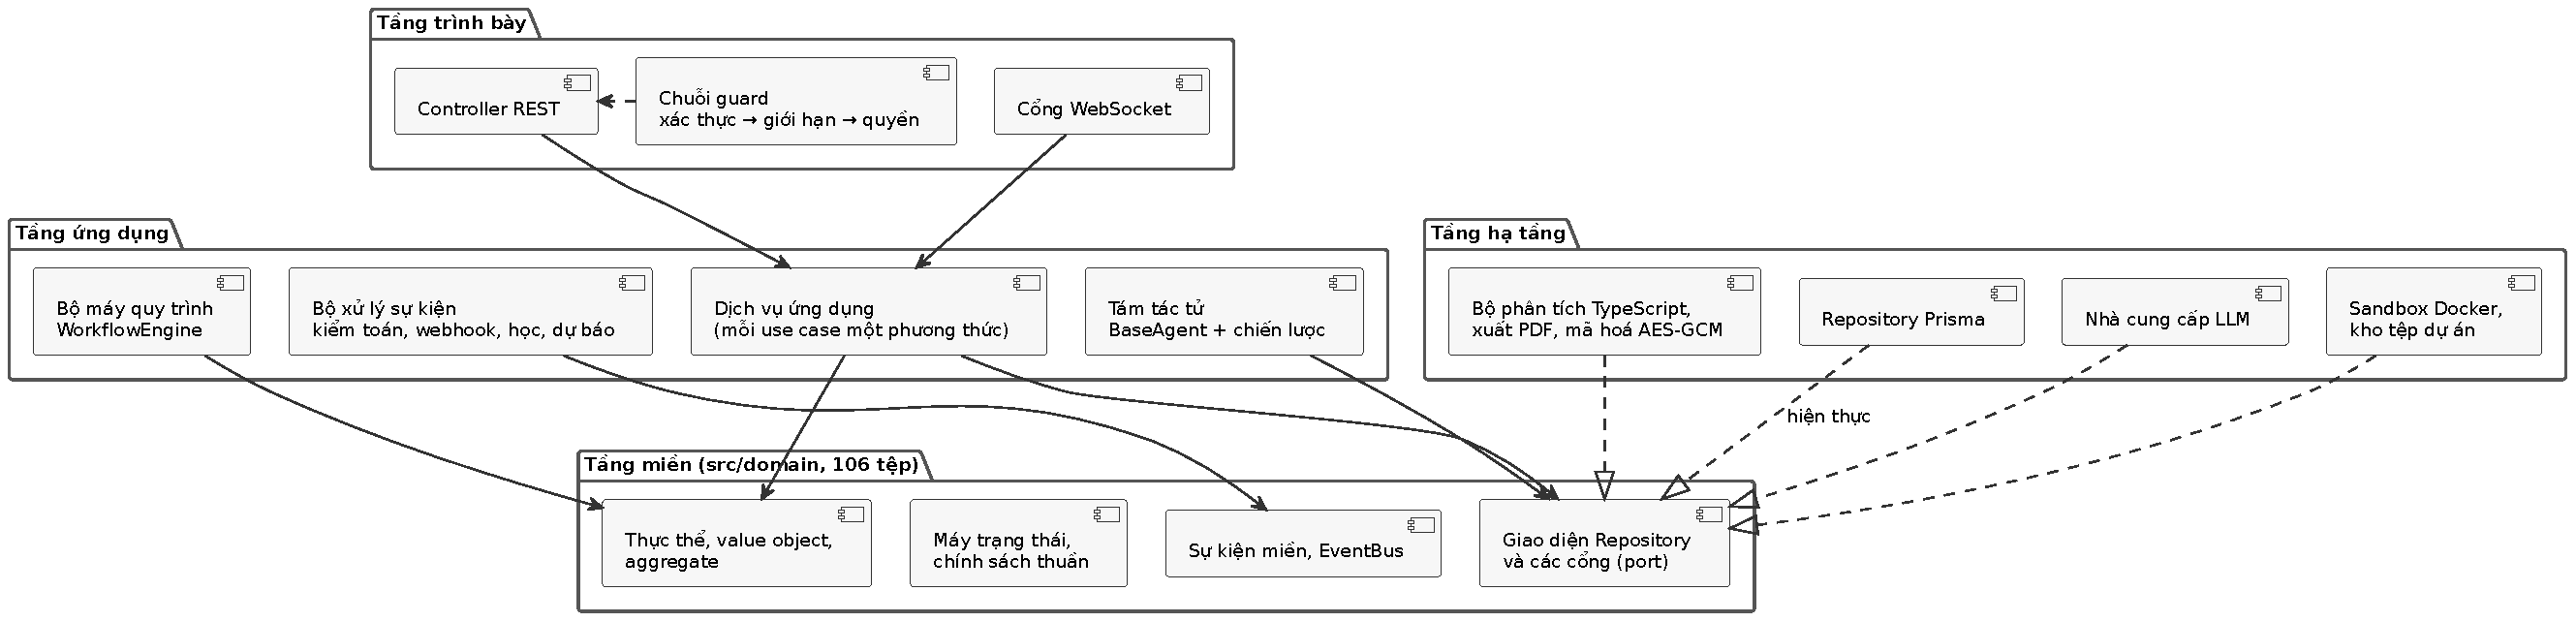
\includegraphics[width=\textwidth]{sodo/kien-truc-phan-lop.pdf}
\end{figure}

\subsection{Các quyết định kiến trúc chính}

Mỗi quyết định kiến trúc được ghi thành một bản ghi quyết định kiến trúc (ADR) trong \code{docs/design/architecture.md}. Sáu quyết định có tác động lớn nhất như sau:

\begin{enumerate}
\item \textbf{Chọn NestJS cho API.} NestJS có sẵn cơ chế tiêm phụ thuộc và hệ thống mô-đun, tức là làm sẵn nguyên lý DIP. Nó còn cho đăng ký nhiều hiện thực dưới cùng một token, và nền tảng tận dụng điều này cho danh sách tác tử và danh sách chiến lược nút.
\item \textbf{Chọn PostgreSQL} cho cả dữ liệu quan hệ lẫn dữ liệu JSON như ngữ cảnh lượt chạy hay siêu dữ liệu OOAD, với Prisma làm lớp ánh xạ nằm sau các Repository.
\item \textbf{Chọn BullMQ trên Redis} làm hàng đợi cho các nút quy trình. Thiếu Redis thì bộ máy chạy nút trực tiếp. Điểm kiểm tra tình trạng khi đó báo \textit{degraded} nhưng hệ thống vẫn chạy.
\item \textbf{Mọi truy cập dữ liệu từ tầng ứng dụng đi qua Repository}, nên dịch vụ ứng dụng kiểm thử được bằng Repository lưu trong bộ nhớ.
\item \textbf{Chuyên môn hoá tác tử bằng Strategy} thay cho cây kế thừa sâu (mục~\ref{sec:tk-tac-tu}).
\item \textbf{Các mô-đun nói chuyện với nhau qua sự kiện miền.} Kiểm toán, webhook, cơ chế học, dự báo và giám sát bất thường đều chỉ nghe sự kiện, không gọi thẳng vào nhau.
\end{enumerate}

\section{Mẫu thiết kế}
\label{sec:mau}

Bảng~\ref{tab:mau-1} và Bảng~\ref{tab:mau-2} ghép mỗi mẫu thiết kế với vấn đề nó giải quyết và lớp hiện thực nó. Lớp nào trong mã cũng có chú thích \code{@pattern}, nên người đọc có thể tìm trong kho mã để so từng dòng của bảng.

\begin{table}{Mẫu thiết kế trong nền tảng (phần 1: tác tử và quy trình)}
\label{tab:mau-1}
\footnotesize
\begin{tabularx}{\textwidth}{|L|P{2.7cm}|P{5.3cm}|}
\hline
\textbf{Vấn đề} & \textbf{Mẫu} & \textbf{Hiện thực} \\ \hline
Tám vai trò có chung chu trình nhận việc, suy nghĩ, hành động, hoàn tất & Template Method & \code{BaseAgent.execute()} \\ \hline
Mỗi vai trò suy nghĩ và hành động khác nhau, cần thay được độc lập & Strategy & \code{IThinkingStrategy}, \code{IActionStrategy}, 16 lớp chiến lược \\ \hline
Thêm vai trò mà không sửa bộ điều phối & Registry + DIP & \code{AgentOrchestrator} nhận danh sách \code{IAgent} qua token \code{AGENTS}; mỗi vai trò một \code{RoleProfile} \\ \hline
Tác tử, công việc, dự án, phê duyệt chỉ được chuyển trạng thái hợp lệ & State & \code{AgentStateMachine}, \code{Task.transitionTo}, value object \code{ProjectStatus} \\ \hline
Nhiều bên cần biết khi tác tử đổi trạng thái hoặc xong việc & Observer & \code{AgentEventEmitter}, \code{IAgentObserver}; \code{EventBus} và các handler \\ \hline
Mỗi loại nút chạy khác nhau, thêm loại nút không sửa bộ máy & Strategy tự đăng ký & \code{NodeExecutionStrategy}: tác tử, quy trình con, cổng chất lượng, điều kiện, song song, phê duyệt, cộng tác \\ \hline
Một nút là cả một quy trình & Composite & \code{SubWorkflowStrategy} chạy quy trình con thành lượt chạy con \\ \hline
Quay lại trạng thái trước của lượt chạy & Memento & \code{WorkflowRunMemento}, \code{WorkflowSnapshotCaretaker} \\ \hline
Định nghĩa quy trình không bị sửa khi đã có lượt chạy dùng nó & Sổ đăng ký bất biến & \code{WorkflowDefinitionRegistry} theo khoá \code{id@phiên_bản+băm} \\ \hline
Tác tử trao đổi thông điệp có kiểu khi cộng tác & Mediator & \code{AgentMessageBus}, \code{EventBus} \\ \hline
\end{tabularx}
\end{table}

\begin{table}{Mẫu thiết kế trong nền tảng (phần 2: LLM, bảo mật, báo cáo, chất lượng)}
\label{tab:mau-2}
\footnotesize
\begin{tabularx}{\textwidth}{|L|P{2.7cm}|P{5.3cm}|}
\hline
\textbf{Vấn đề} & \textbf{Mẫu} & \textbf{Hiện thực} \\ \hline
Ghi chi phí mọi lời gọi LLM mà không sửa nhà cung cấp & Decorator & \code{UsageTrackingLLMProvider} \\ \hline
Tác tử gọi LLM qua một cửa duy nhất & Facade & \code{AgentLLMService}, \code{OoadArtifactService}, \code{CodeQualityService} \\ \hline
Nhiều nhà cung cấp LLM sau một giao diện & Adapter + Factory Method & \code{ILLMProvider}, \code{LLMProviderFactory} \\ \hline
Quản trị viên thêm nhà cung cấp, mô hình lúc hệ thống đang chạy & Aggregate + Strategy + Registry & \code{LlmProviderConfig} chứa \code{LlmModel}; \code{ProviderStrategy} cho mỗi loại; \code{ProviderStrategyRegistry}, \code{ConfiguredProviderRegistry} \\ \hline
Mã hoá khoá API của nhà cung cấp mà tầng miền không phụ thuộc thư viện mật mã & Port/Adapter & \code{SecretCipher} (miền), \code{AesGcmSecretCipher} (hạ tầng) \\ \hline
Một phê duyệt chỉ được trả lời một lần dù có hai yêu cầu đồng thời & Cập nhật có điều kiện & \code{ApprovalService}: chỉ cập nhật khi trạng thái còn \code{pending} \\ \hline
Xác thực, giới hạn tần suất rồi mới kiểm tra quyền & Chain of Responsibility & \code{AuthenticationGuard}, \code{RateLimitGuard}, \code{PermissionGuard}; chuỗi rà soát QC rồi QA \\ \hline
Biến sự kiện miền thành mục kiểm toán hoặc payload webhook & Adapter & \code{AuditLogHandler}, \code{webhook-payloads} \\ \hline
Tách truy cập dữ liệu khỏi miền & Repository, Data Mapper & \code{I*Repository} ở miền, \code{Prisma*Repository} ở hạ tầng \\ \hline
Dựng báo cáo chi phí, hiệu năng theo từng bước & Builder & \code{CostReportBuilder}, \code{PerformanceReportBuilder} \\ \hline
Xuất JSON, CSV, PDF tuỳ định dạng & Strategy + Registry & \code{ProjectExportService} và ba exporter \\ \hline
Mỗi loại bất thường, mỗi tín hiệu chất lượng là một quy tắc & Strategy + Composite & \code{IAgentAnomalyRule}, \code{IQualitySignal}, \code{AgentAnomalyDetector} \\ \hline
Phân tích mã sinh ra mà miền không phụ thuộc trình biên dịch & Port/Adapter & \code{ICodeAnalyzer} (miền), \code{TypeScriptCodeAnalyzer} (hạ tầng) \\ \hline
Quy tắc chấm điểm chất lượng mã & Policy, Specification & \code{CodeQualityPolicy}, \code{LayerRules} \\ \hline
\end{tabularx}
\end{table}

\section{Thiết kế tác tử}
\label{sec:tk-tac-tu}

\subsection{Một khung chung, hai chiến lược riêng}

Mỗi tác tử là một đối tượng \code{BaseAgent} lắp từ ba phần (Hình~\ref{fig:lop-tac-tu}). Phần thứ nhất là \code{RoleProfile}, mô tả vai trò, các loại công việc vai trò làm được và lời nhắc hệ thống. Hai phần còn lại là một chiến lược tư duy và một chiến lược hành động. Phương thức \code{BaseAgent.execute()} giữ cố định khung thuật toán như sau:

\begin{enumerate}
\item Chuẩn hoá ngữ cảnh. Loại công việc được so với hồ sơ vai trò, nên chiến lược lúc nào cũng nhận đúng loại việc mà vai trò đó làm được.
\item Phát sự kiện \code{TaskAssignedEvent}.
\item Chuyển \code{IDLE} sang \code{THINKING} rồi gọi \code{thinkingStrategy.think(context)}. Ở bước này, chiến lược nạp bộ nhớ, nạp bài học liên quan và gọi LLM để lập kế hoạch.
\item Chuyển \code{THINKING} sang \code{ACTING} rồi gọi \code{actionStrategy.act(context, thought)}. Chiến lược sinh tài liệu hoặc mã, ghi vào kho tệp của dự án và chạy các công cụ cần thiết.
\item Chuyển sang \code{COMPLETED} rồi về \code{IDLE}, lưu ký ức và phát \code{AgentCompletedTaskEvent}.
\item Nếu có ngoại lệ, tác tử chuyển sang \code{ERROR}. Với lỗi tạm thời, tác tử được quay về \code{IDLE}.
\end{enumerate}

\begin{figure}{Sơ đồ lớp của tác tử: Template Method kết hợp hai Strategy}
\label{fig:lop-tac-tu}
\centering
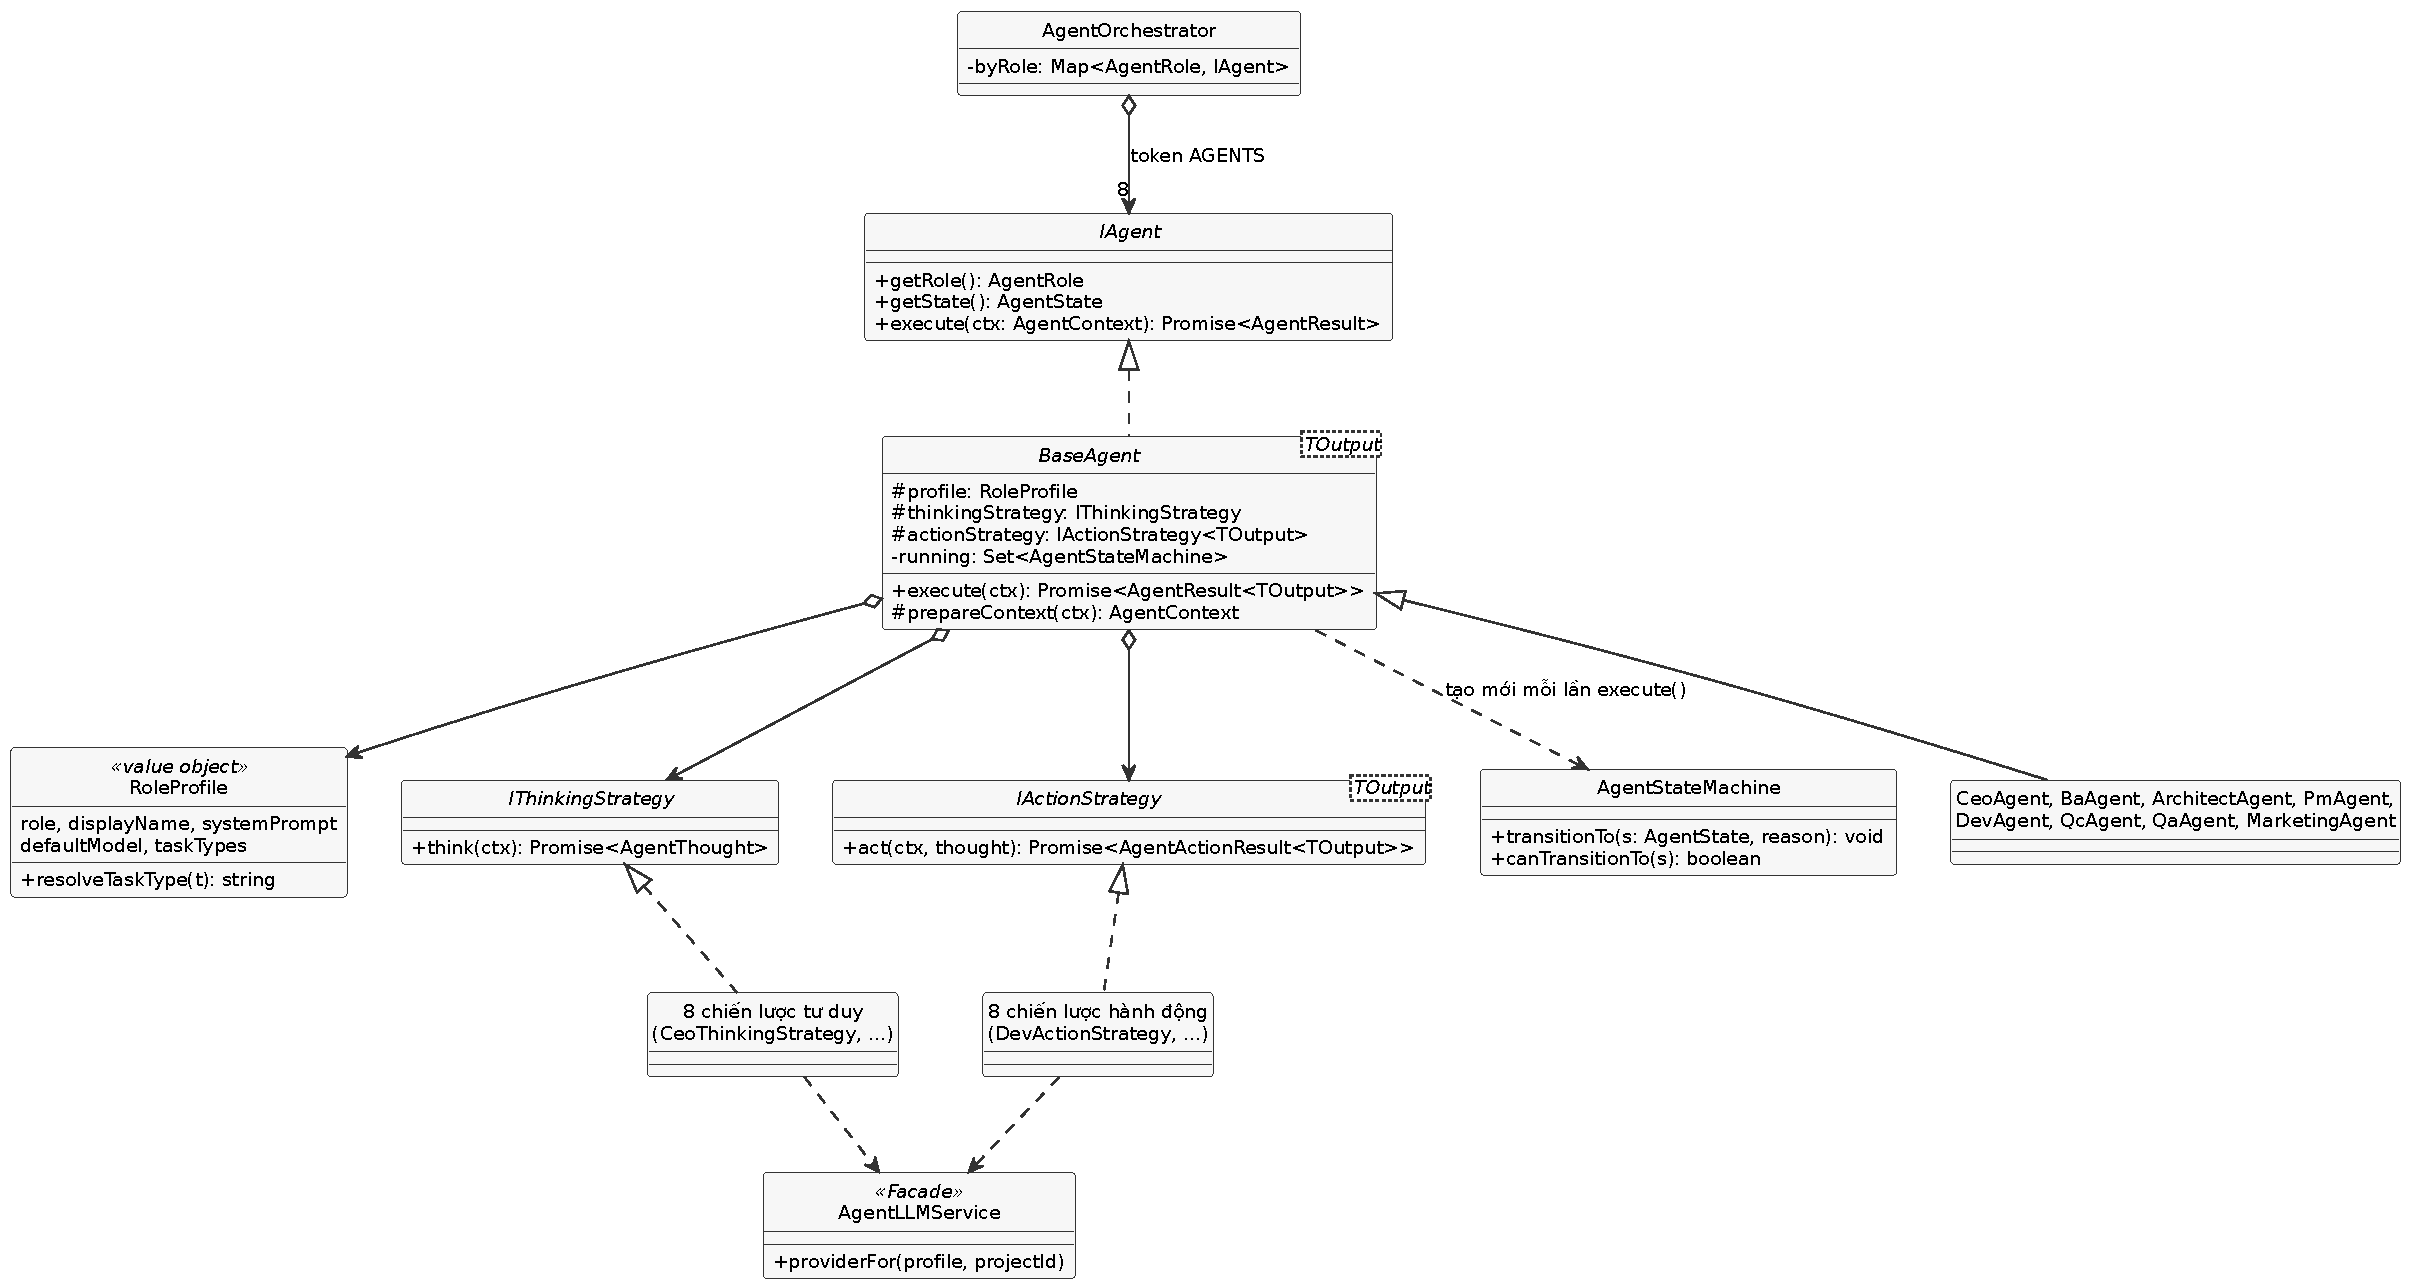
\includegraphics[width=\textwidth]{sodo/lop-tac-tu.pdf}
\end{figure}

Chia như vậy thì thoả ba nguyên lý SOLID. Tác tử chỉ lo vòng đời, chuyên môn để trong chiến lược, nên lớp nào cũng chỉ có một lý do để sửa (SRP). Muốn thêm vai trò thì thêm một hồ sơ và hai chiến lược, không phải đụng vào mã cũ (OCP). Mọi tác tử đều thay thế được cho nhau qua giao diện \code{IAgent}, nên bộ điều phối không cần biết mình đang gọi CEO hay QC (LSP).

\subsection{Máy trạng thái gắn với từng lần thực thi}

Thiết kế ban đầu cho mỗi vai trò giữ đúng một máy trạng thái. Lúc kiểm thử, cách này gây ra hai chuyện. Một là khi hai công việc cùng vai trò chạy song song, chúng ghi đè trạng thái của nhau và sinh lỗi ``Invalid state transition: IDLE → ERROR''. Hai là sau một lỗi không phục hồi được, vai trò đó kẹt luôn ở \code{ERROR} và từ chối mọi việc giao sau đó.

Sau khi sửa, mỗi lần gọi \code{execute()} có một máy trạng thái riêng. Tác tử giữ tập các máy trạng thái đang chạy và báo ra trạng thái của lần thực thi gần nhất (Hình~\ref{fig:sm-tac-tu}). Bài học ở đây về mẫu State là máy trạng thái phải gắn với thứ thật sự có vòng đời, ở đây là một lần thực thi, chứ không gắn vào một đối tượng sống lâu như chính tác tử.

\begin{figure}{Máy trạng thái của một lần thực thi tác tử}
\label{fig:sm-tac-tu}
\centering
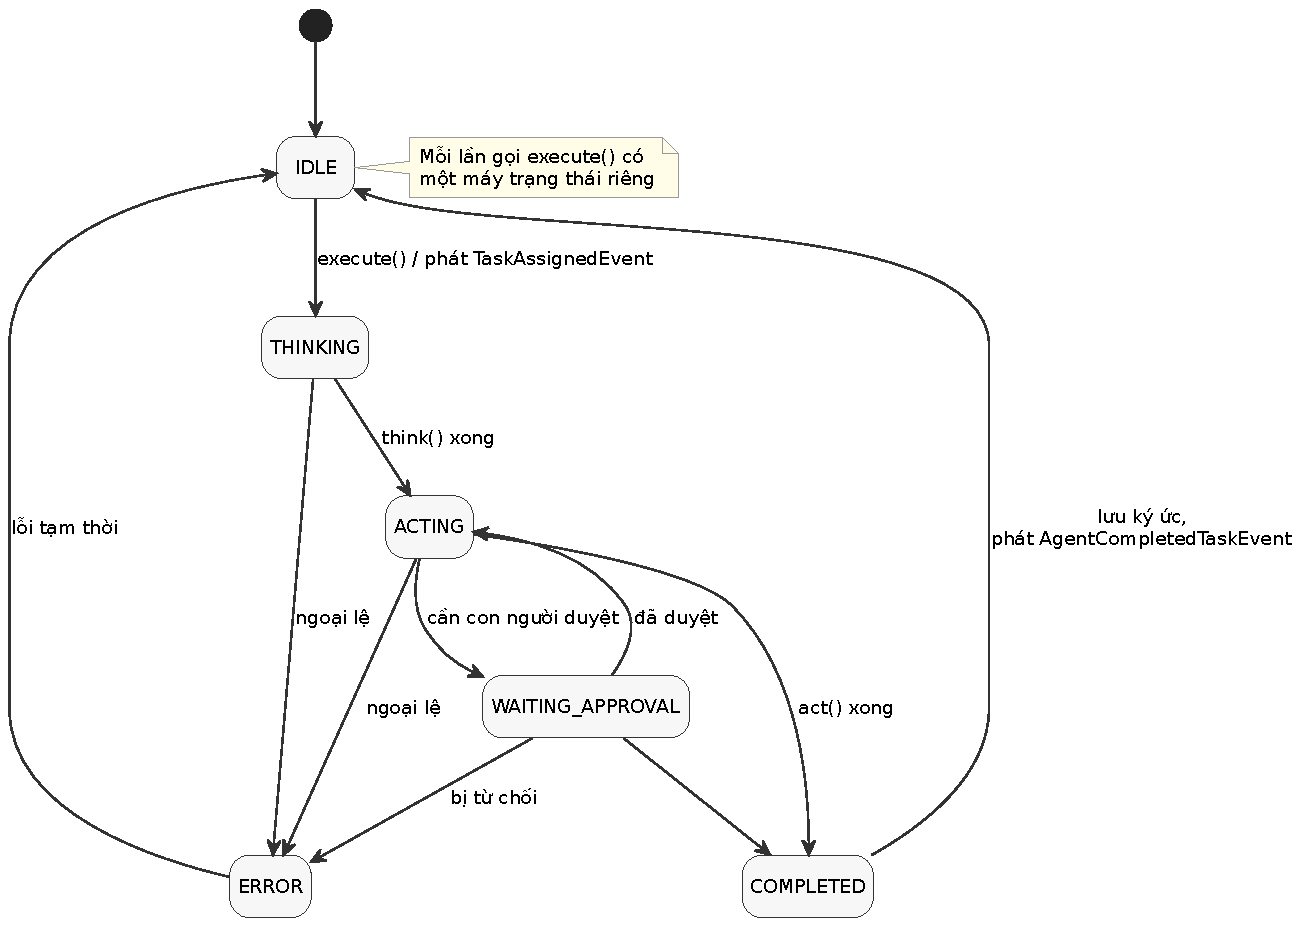
\includegraphics[width=0.78\textwidth]{sodo/may-trang-thai-tac-tu.pdf}
\end{figure}

\subsection{Gọi LLM và ghi chi phí}
\label{subsec:llm}

Chiến lược không gọi thẳng nhà cung cấp LLM mà đi qua \code{AgentLLMService}, một Facade. Lớp này tra cấu hình mô hình của vai trò, lấy nhà cung cấp từ \code{LLMProviderFactory}, rồi bọc nhà cung cấp trong \code{UsageTrackingLLMProvider} theo mẫu Decorator. Decorator chuyển nguyên lời gọi xuống lớp bên trong. Có kết quả rồi, nó ghi số token và chi phí vào \code{ApiUsageLog}, cộng vào chi phí dự án và phát \code{BudgetExceededEvent} đúng một lần khi vượt ngân sách. Nhờ thế chi phí của cả tám vai trò đều được ghi đủ, và không chiến lược nào phải tự tính tiền.

Nhà cung cấp và mô hình LLM được quản lý ngay trong ứng dụng, bên cạnh cách cấu hình bằng biến môi trường (Hình~\ref{fig:lop-llm}). \code{LlmProviderConfig} là gốc aggregate. Nó quản lý danh sách \code{LlmModel}, tự kiểm tra các bất biến (tên dài từ 1 đến 60 ký tự, URL http hoặc https hợp lệ, loại nhà cung cấp đã được hỗ trợ, không trùng mô hình) và chỉ lưu khoá API ở dạng đã mã hoá. Việc mã hoá đi qua cổng \code{SecretCipher} của tầng miền, còn tầng hạ tầng hiện thực cổng này bằng AES-256-GCM với khoá \code{LLM_SECRET_KEY}. API chỉ trả về bốn ký tự cuối của khoá. Mỗi loại nhà cung cấp, hiện là tương thích OpenAI và Anthropic, là một \code{ProviderStrategy} biết tạo client, kiểm tra kết nối và lấy danh sách mô hình. Muốn hỗ trợ thêm loại mới thì chỉ việc thêm một chiến lược vào sổ đăng ký.

Cấu hình mô hình của mỗi vai trò có thêm trường \code{providerId}. \code{LLMProviderFactory} hỏi \code{ConfiguredProviderRegistry} để lấy client đã cấu hình (có bộ đệm), hoặc dùng cổng mặc định khi vai trò chưa chọn nhà cung cấp. Lần khởi động đầu tiên, nếu bảng nhà cung cấp còn trống, hệ thống lấy cổng LLM khai báo trong biến môi trường làm nhà cung cấp đầu tiên, để bản cài đặt cũ khỏi phải cấu hình lại. Khi thêm tính năng này, tác tử, chiến lược và decorator ghi chi phí không phải sửa dòng nào, vì chúng chỉ biết tới giao diện \code{ILLMProvider}.

\begin{figure}{Sơ đồ lớp của phần quản lý nhà cung cấp LLM}
\label{fig:lop-llm}
\centering
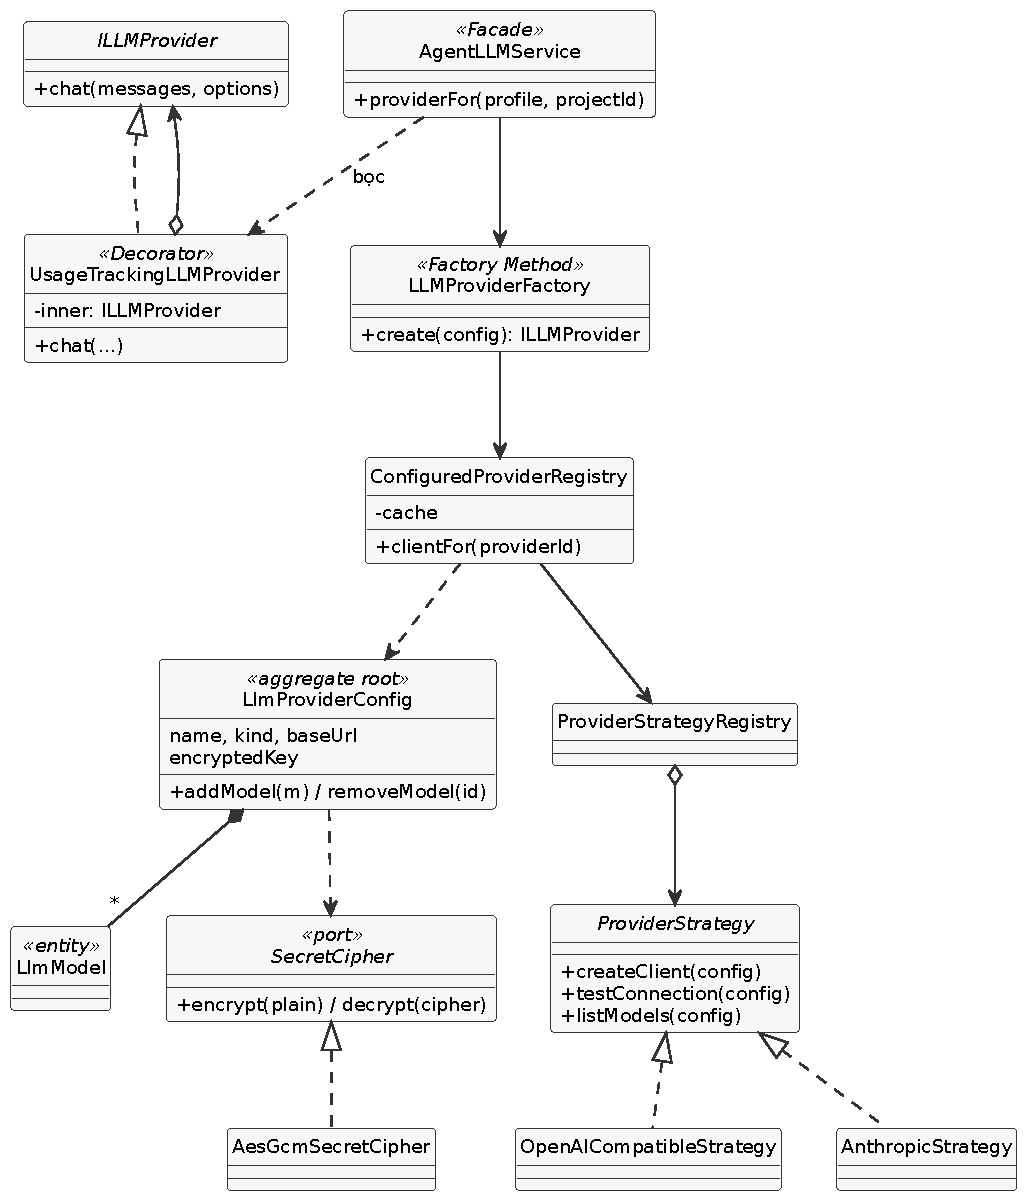
\includegraphics[width=0.72\textwidth]{sodo/lop-nha-cung-cap-llm.pdf}
\end{figure}

\subsection{Học từ kết quả}
\label{subsec:hoc}

Cơ chế học gồm ba phần (Hình~\ref{fig:tuan-tu-hoc}):

\begin{enumerate}
\item \code{OutcomeSignalPolicy} là một chính sách thuần, quyết định tín hiệu nào dùng để chấm lần thực thi nào. Kết quả cổng OOAD dùng để chấm BA và Architect. Kết quả của QC (số kiểm thử đạt, use case còn thiếu) dùng để chấm DEV. Phán quyết của QA chấm cả DEV và QC.
\item \code{LearningService} lưu từng kết quả vào bộ nhớ của vai trò. Cứ đủ N kết quả (mặc định là 3), dịch vụ gọi LLM để tóm các kết quả gần đây lại thành một ký ức loại \code{lessons_learned}. Lời gọi này cũng bị tính tiền như mọi lời gọi khác.
\item Khi dựng lời nhắc, chiến lược tư duy nạp các bài học này trước tiên.
\end{enumerate}

\begin{figure}{Tuần tự của chu trình học từ kết quả}
\label{fig:tuan-tu-hoc}
\centering
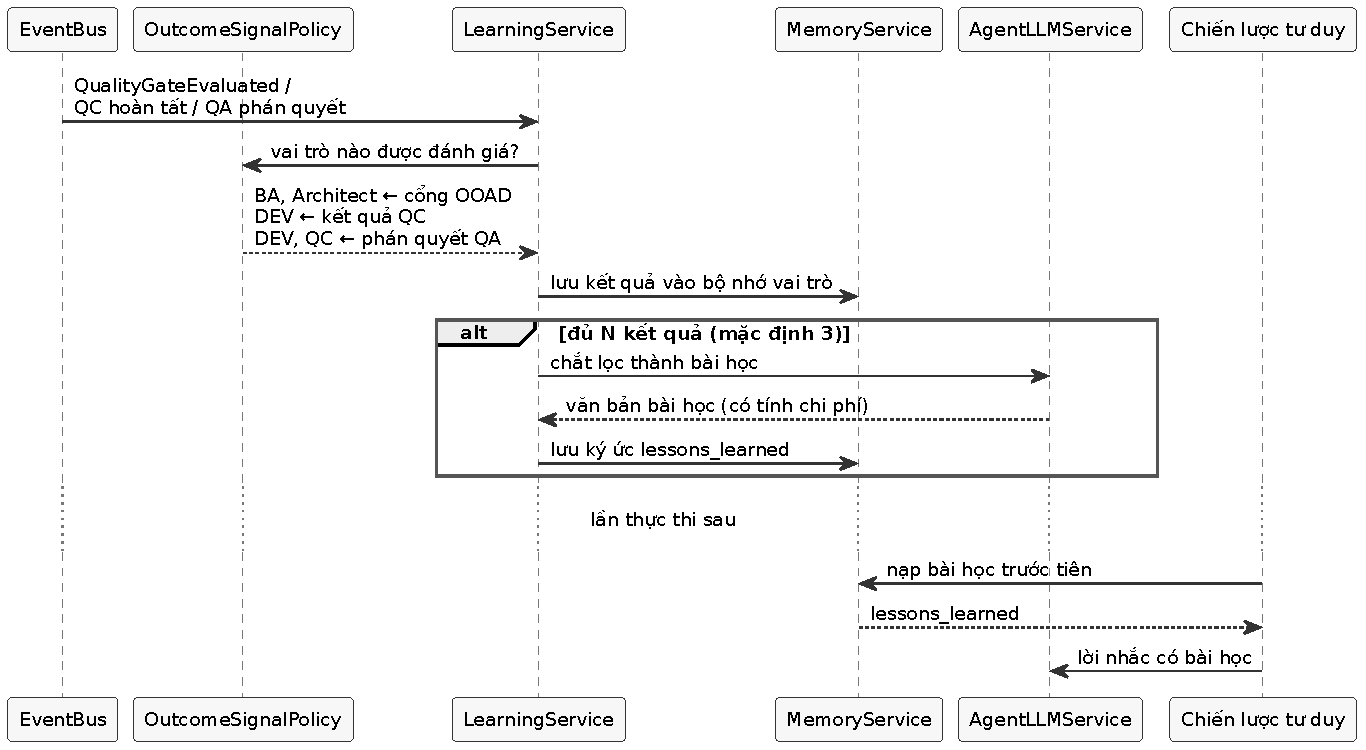
\includegraphics[width=0.85\textwidth]{sodo/tuan-tu-hoc.pdf}
\end{figure}

Thiết kế này giống Reflexion~\cite{shinn2023} ở chỗ phản hồi được viết bằng lời. Chỗ khác là tín hiệu chấm điểm đến từ một nguồn khách quan bên ngoài tác tử, còn ở Reflexion tác tử tự chấm chính mình.

\subsection{Cộng tác giữa các tác tử}

Có ba kiểu cộng tác. Mỗi kiểu là chiến lược của một nút quy trình và được đăng ký trong \code{CollaborationRegistry}:

\begin{itemize}
\item \textbf{Lập trình cặp} (\code{pair_develop}). DEV lập kế hoạch, chỗ nào trong use case còn mơ hồ thì hỏi BA trước. Sau đó DEV gửi thông điệp \code{PROPOSE}, Architect trả lời \code{ACCEPT} hoặc \code{REJECT} kèm góp ý. DEV viết mã xong thì Architect rà soát lại. Số vòng trao đổi bị giới hạn để chi phí không vượt mức cho phép.
\item \textbf{Vòng làm rõ} (\code{clarification_loop}). Tác tử hỏi BA và chờ câu trả lời trước khi làm tiếp.
\item \textbf{Chuỗi rà soát} (\code{review_chain}), theo mẫu Chain of Responsibility. QC xem trước, QA xem sau, và chỉ cần một mắt xích từ chối là chuỗi dừng.
\end{itemize}

Mọi lượt trao đổi đều đi qua \code{AgentMessageBus} theo mẫu Mediator, dùng các performative theo tinh thần FIPA-ACL~\cite{fipa2002}. Người dùng theo dõi chúng ở màn hình Phòng họp (Meeting Room). Hình~\ref{fig:meeting-room} chụp lúc một dự án mới đang chạy: bên trái là trạng thái tám tác tử, bên phải là các bước suy nghĩ mà từng tác tử gửi cho cả nhóm.

\begin{figure}{Văn phòng ảo và Phòng họp trong lúc dự án đang chạy}
\label{fig:meeting-room}
\centering
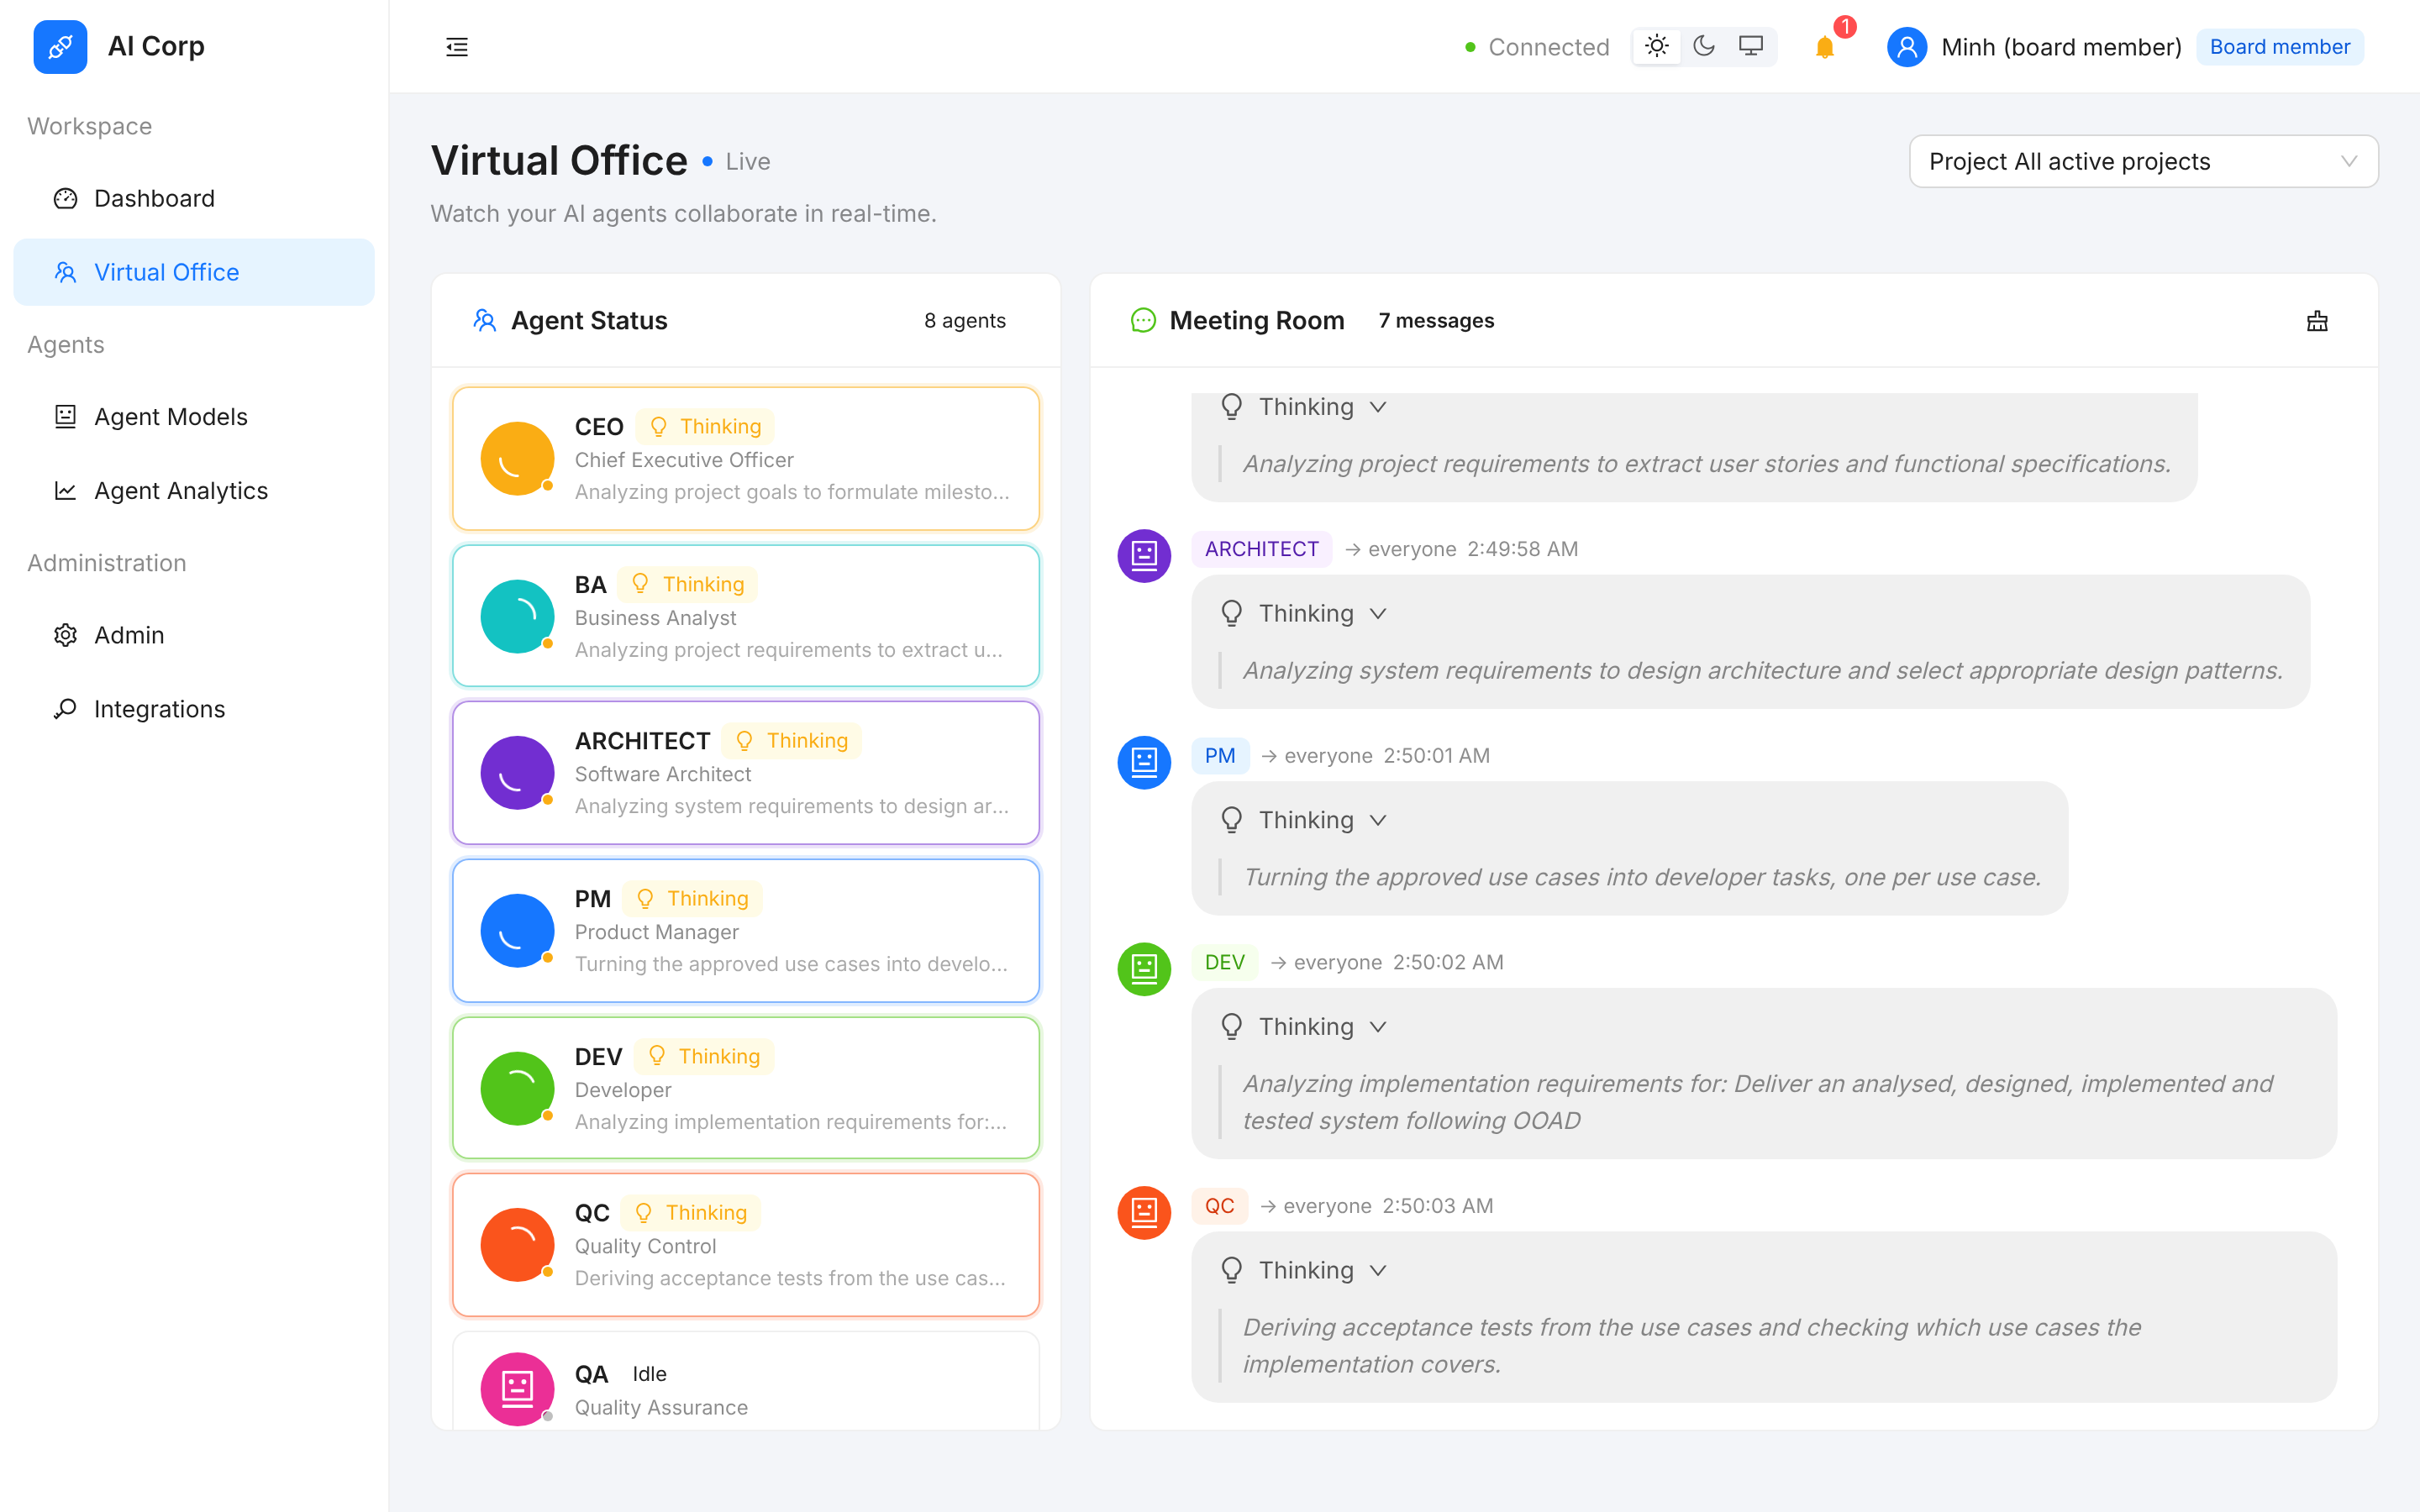
\includegraphics[width=\textwidth]{anh/meeting-room.png}
\end{figure}

\section{Thiết kế bộ máy quy trình}
\label{sec:bo-may}

\subsection{Định nghĩa và thực thi}

Một quy trình là một đồ thị gồm các nút có kiểu và các cạnh. Cạnh có thể là cạnh mặc định, cạnh có điều kiện hoặc cạnh \code{onFail}. \code{WorkflowEngine} không chứa logic riêng của loại nút nào. Mỗi loại nút là một \code{NodeExecutionStrategy} tự đăng ký vào bộ máy (Hình~\ref{fig:lop-bo-may}). Muốn thêm loại nút mới, chẳng hạn cổng chất lượng, chỉ cần viết thêm một lớp mà không phải sửa vòng lặp thực thi. Đó chính là nguyên lý OCP.

\begin{figure}{Sơ đồ lớp của bộ máy quy trình}
\label{fig:lop-bo-may}
\centering
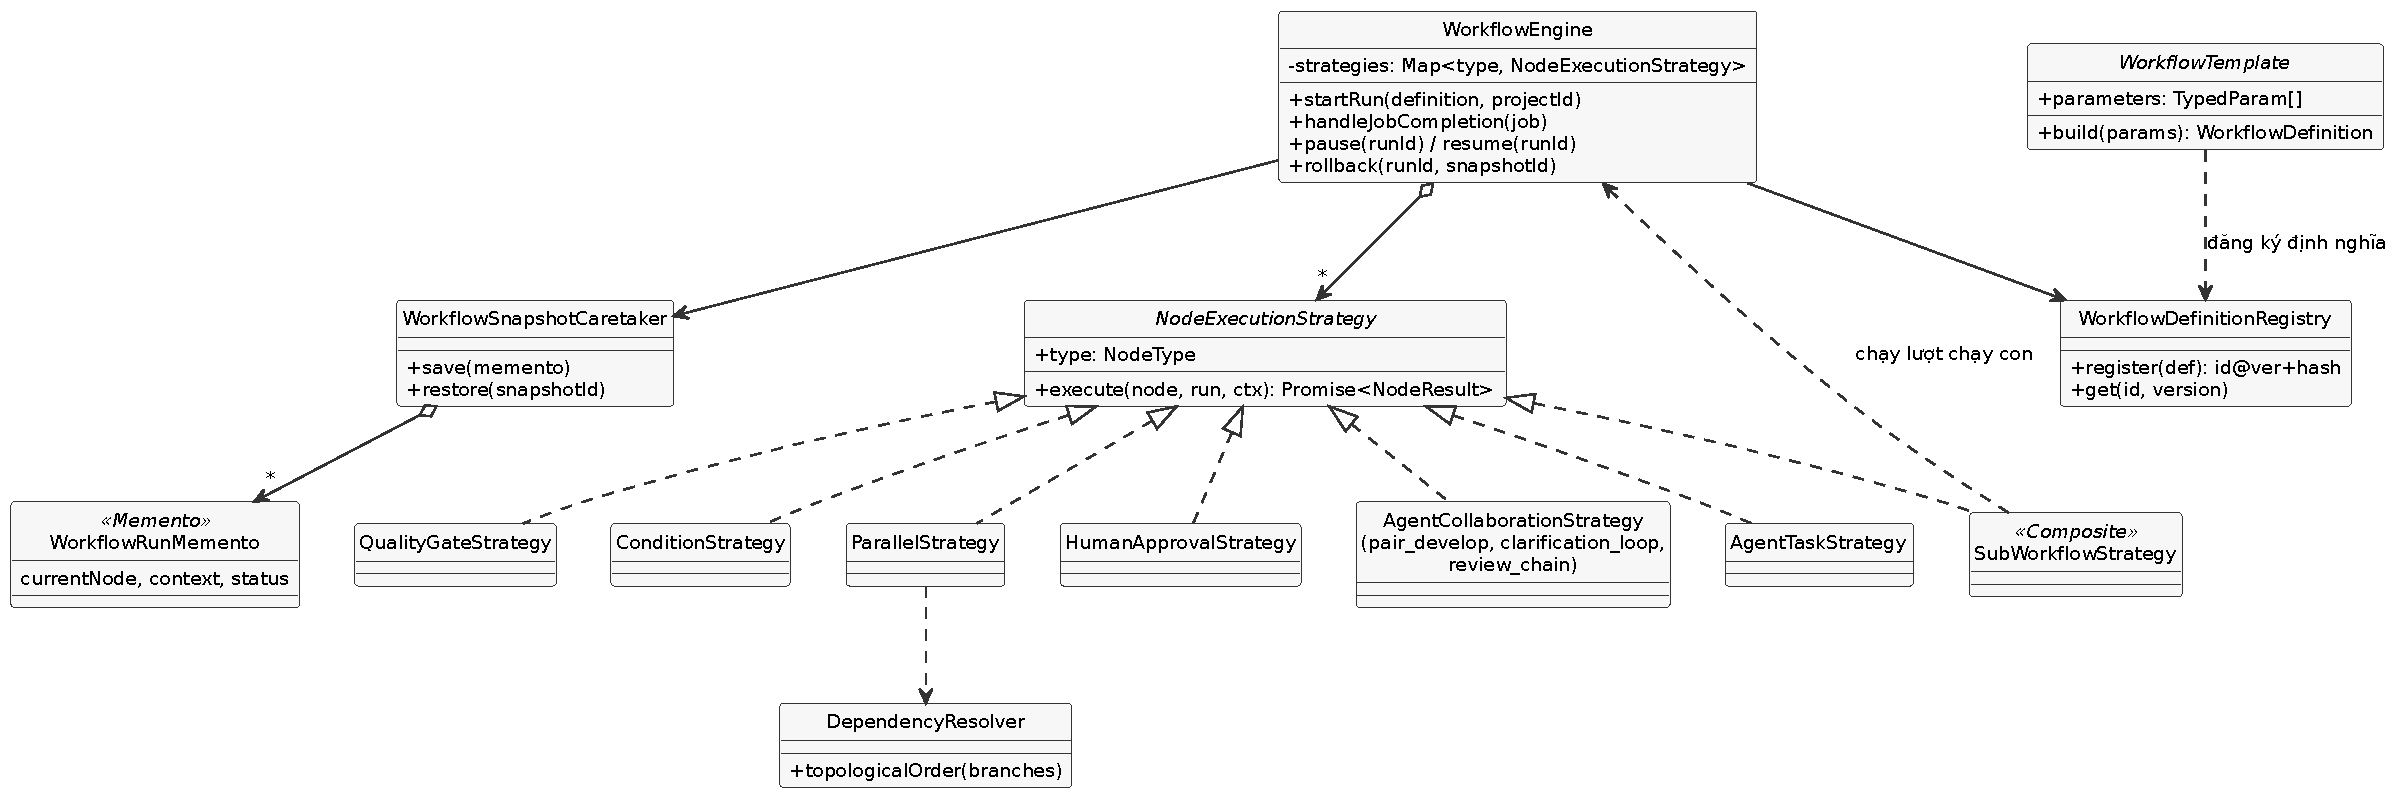
\includegraphics[width=\textwidth]{sodo/lop-bo-may-quy-trinh.pdf}
\end{figure}

Hình~\ref{fig:quy-trinh} là quy trình mặc định cho một dự án phần mềm. Quy trình này có hai quy trình con, mỗi cái có một vòng lặp. Vòng thiết kế quay lại Architect khi cổng OOAD không đạt, còn vòng xây dựng quay lại DEV khi QA từ chối.

\begin{figure}{Quy trình mặc định của một dự án phần mềm OOAD}
\label{fig:quy-trinh}
\centering
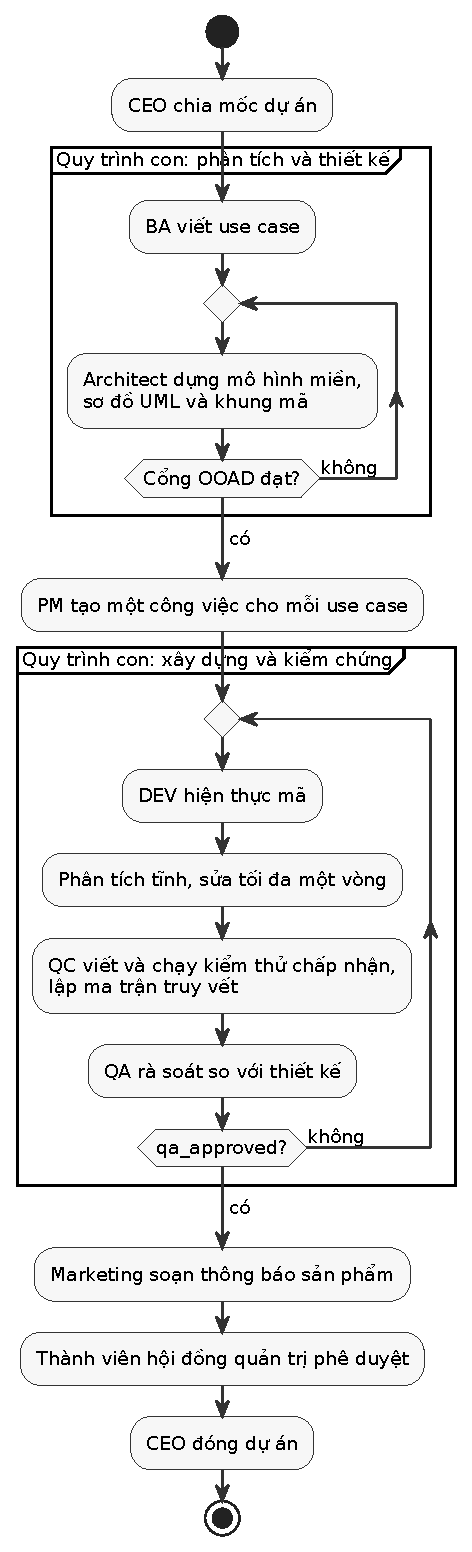
\includegraphics[height=0.62\textheight]{sodo/quy-trinh-mac-dinh.pdf}
\end{figure}

Hình~\ref{fig:tuan-tu-nut} cho thấy một nút tác tử đi qua những lớp nào. Bộ máy kiểm tra ngân sách trước, đẩy công việc vào hàng đợi, chiến lược nút gọi tác tử, tác tử gọi LLM qua Facade và Decorator. Khi nút xong, bộ máy ghi bước, chụp memento và chọn cạnh kế tiếp.

\begin{figure}{Tuần tự xử lý một nút tác tử}
\label{fig:tuan-tu-nut}
\centering
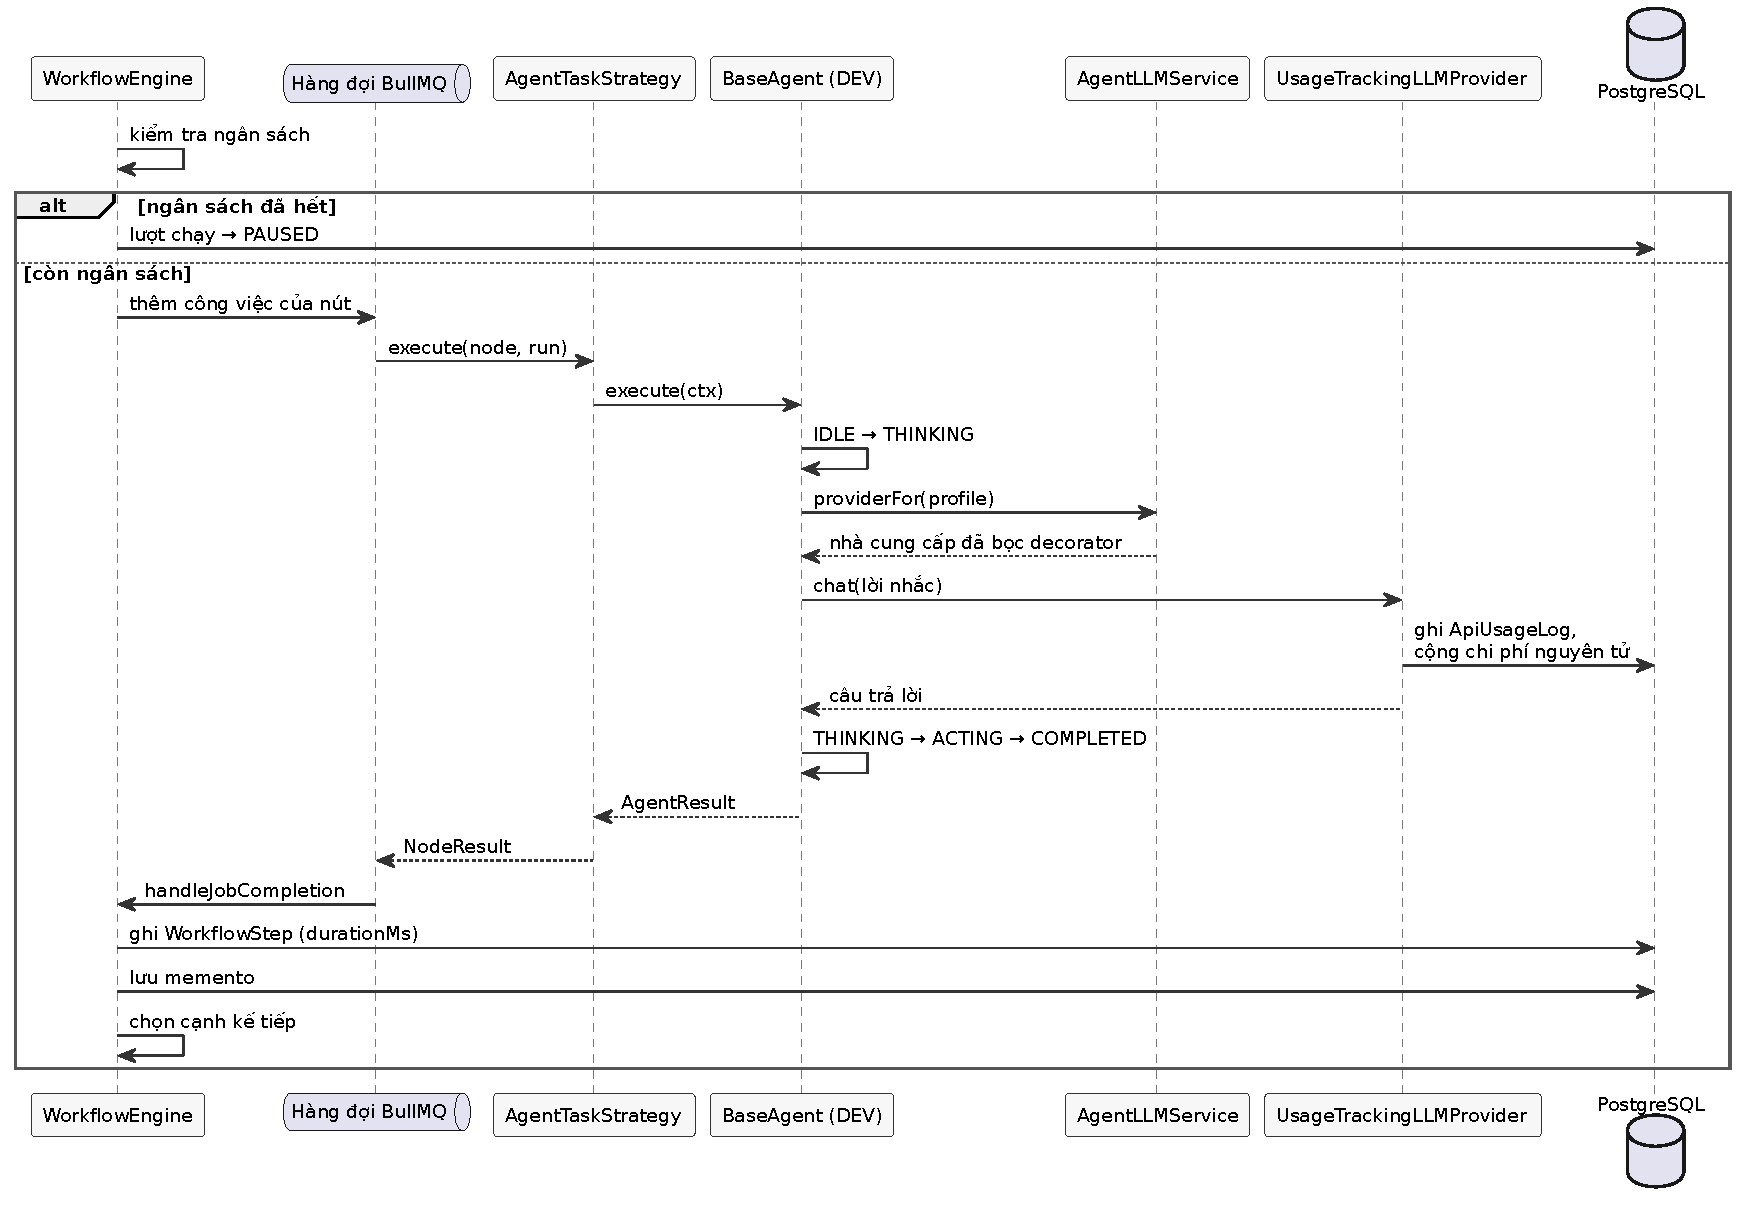
\includegraphics[width=\textwidth]{sodo/tuan-tu-thuc-thi-nut.pdf}
\end{figure}

\subsection{Quy trình con, phiên bản và khôi phục}

\begin{itemize}
\item \textbf{Quy trình con (Composite).} Nút \code{sub_workflow} chạy một quy trình khác thành lượt chạy con có \code{parentRunId}. Kết quả của lượt chạy con được gộp vào ngữ cảnh của lượt chạy cha. Ba mẫu quy trình có kiểu (dự án phần mềm OOAD, backend REST API, chỉ phân tích và thiết kế) dùng chung các quy trình con này.
\item \textbf{Phiên bản bất biến.} Mỗi định nghĩa quy trình được lưu theo khoá \code{id@phiên_bản} cùng mã băm của nội dung đã chuẩn hoá. Đăng ký lại cùng phiên bản với nội dung khác sẽ bị từ chối, và mỗi lượt chạy gắn cố định với một phiên bản.
\item \textbf{Ảnh chụp và khôi phục (Memento).} Sau mỗi nút, \code{WorkflowSnapshotCaretaker} lưu một memento gồm nút hiện tại, ngữ cảnh và trạng thái. Người dùng có thể đưa một lượt chạy đang tạm dừng về một ảnh chụp trước đó. Khi ấy các yêu cầu phê duyệt còn treo phát sinh sau ảnh chụp sẽ bị huỷ.
\item \textbf{Song song có phụ thuộc.} Nút \code{parallel} chạy các nhánh theo thứ tự tô-pô xác định bởi \code{dependsOn}, có giới hạn số nhánh chạy cùng lúc. \code{DependencyResolver} lo việc phát hiện chu trình phụ thuộc.
\end{itemize}

\subsection{Xử lý lỗi}

Nút lỗi được thử lại tối đa ba lần, mỗi lần chờ lâu gấp đôi lần trước. Vẫn lỗi thì lượt chạy đi theo cạnh \code{onFail} nếu có, còn không thì chuyển sang \code{failed} và phát \code{workflow.failed}. Kiểm thử đã lôi ra hai lỗi thiết kế ở đúng chỗ này. Trước khi sửa, một nút lỗi có thể làm lượt chạy kẹt mãi ở \code{running}, hoặc ngược lại cho lượt chạy đi tiếp theo cạnh thành công như chưa hề có lỗi.

\subsection{Điều khiển lượt chạy và ngân sách}

Các thao tác tạm dừng, tiếp tục và huỷ tác động lên lượt chạy mới nhất của dự án chứ không chỉ đổi trạng thái dự án. Xoá dự án thì lượt chạy bị huỷ và kho tệp cũng bị xoá theo. Có ba quy tắc giữ cho các thao tác này chạy đúng:

\begin{itemize}
\item Không cho tiếp tục khi lượt chạy đang chờ phê duyệt, vì nút phê duyệt sẽ chạy lại và sinh ra yêu cầu phê duyệt thứ hai. Cũng không cho tiếp tục khi ngân sách đã hết. Cả hai trường hợp đều trả lỗi kèm lý do.
\item Không nút nào được bắt đầu khi ngân sách đã hết. Bộ máy kiểm tra ngân sách trước mỗi nút và tạm dừng lượt chạy nếu cần. Chi phí được cộng bằng phép tăng nguyên tử trong cơ sở dữ liệu thay cho kiểu đọc rồi ghi. Thông báo ở mức 90\% và 100\% chỉ phát một lần, đúng lúc vượt ngưỡng.
\item Nút nào đã chạy xong trong lúc lượt chạy bị tạm dừng thì không chạy lại khi tiếp tục.
\end{itemize}

Ba quy tắc này có được sau đợt rà soát mã giao diện và logic. Trước đó, nút \textit{Pause} trên giao diện chỉ đổi trạng thái dự án trong khi lượt chạy vẫn chạy tiếp, còn ngân sách chỉ được kiểm tra sau khi tiền đã tiêu. Hình~\ref{fig:sm-luot-chay} tổng hợp các trạng thái của lượt chạy sau khi sửa.

\begin{figure}{Máy trạng thái của lượt chạy quy trình}
\label{fig:sm-luot-chay}
\centering
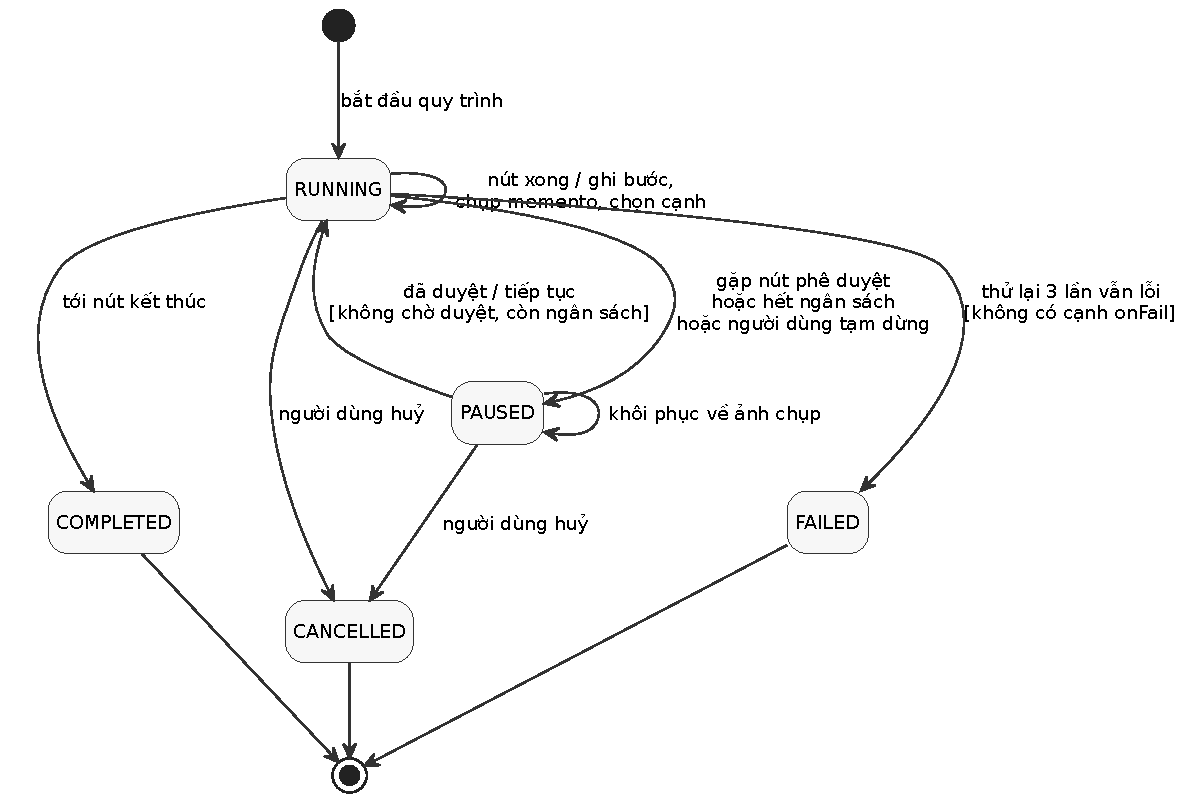
\includegraphics[width=0.8\textwidth]{sodo/may-trang-thai-luot-chay.pdf}
\end{figure}

\section{Thiết kế dữ liệu và lưu trữ}

Dữ liệu có cấu trúc nằm trong PostgreSQL qua 22 mô hình Prisma: người dùng, dự án, mốc, công việc, tác tử, bộ nhớ, lượt chạy, bước, ảnh chụp, phiên bản định nghĩa, phê duyệt, nhật ký sử dụng API, nhật ký cổng chất lượng, nhật ký kiểm toán, khoá API, webhook, lần gửi webhook, dự báo, nhà cung cấp LLM, mô hình LLM và một số bảng khác. Lược đồ được quản lý bằng migration có phiên bản. Một bước kiểm tra riêng so lược đồ dựng từ migration với mô hình Prisma để bắt sai lệch.

Sản phẩm của tác tử (tài liệu, sơ đồ, mã, kiểm thử, báo cáo) không nằm trong cơ sở dữ liệu mà nằm trong \code{ProjectWorkspace}, một thư mục lâu dài cho mỗi dự án. Mọi đường dẫn ghi vào đều được kiểm tra để không thoát ra ngoài thư mục đó, nên một đường dẫn kiểu \code{../../etc/...} do LLM đề xuất sẽ bị từ chối. Ở thiết kế cũ, sản phẩm được ghi vào sandbox Docker, mà sandbox chạy mỗi lệnh trong một container mới không gắn ổ đĩa, nên tệp mất ngay sau mỗi lệnh. Cũng vì vậy mà cổng chất lượng và bước quét kiểm thử của bản cũ chưa lần nào chạy được.

\section{Áp dụng OOAD cho dự án sinh ra}
\label{sec:ooad-du-an}

Dự án nào do nền tảng sinh ra cũng đi qua cùng một chuỗi OOAD, và mắt xích nào trong chuỗi cũng được kiểm tra tự động (Hình~\ref{fig:chuoi-ooad}).

\subsection{Chuỗi sản phẩm}

Bảng~\ref{tab:chuoi-sp} liệt kê sản phẩm của từng bước. Khung mã được dựng từ các mẫu Handlebars theo đúng bốn tầng. Giao diện Repository nằm ở tầng miền, phần hiện thực nằm ở tầng hạ tầng, còn tệp \code{composition-root.ts} ráp các phụ thuộc lại với nhau. Nói cách khác, nền tảng đòi hỏi ở sản phẩm đúng cái kiến trúc mà nó tự áp cho mình.

\begin{table}{Chuỗi sản phẩm OOAD của một dự án sinh ra}
\label{tab:chuoi-sp}
\small
\begin{tabularx}{\textwidth}{|P{2.6cm}|P{2cm}|L|}
\hline
\textbf{Bước} & \textbf{Thực hiện} & \textbf{Sản phẩm trong kho tệp dự án} \\ \hline
Yêu cầu & BA & \code{docs/use-cases.md} \\ \hline
Mô hình miền và UML & Architect & \code{docs/domain-model.puml}, \code{docs/use-case-diagram.puml}, \code{docs/class-diagram.puml}, \code{docs/sequence-UC-xxx.puml}, \code{docs/architecture-patterns.md}, \code{ARCHITECTURE.md} \\ \hline
Khung mã & Architect & \texttt{src/domain/\{entities, value-objects, repositories\}}, \code{src/application/services}, \code{src/infrastructure/persistence}, \code{src/presentation/controllers}, \code{src/composition-root.ts} \\ \hline
Hiện thực & DEV & Mã đầy đủ trong khung, có chú thích \code{UC-xxx} \\ \hline
Chất lượng mã & Hệ thống & \code{docs/code-quality.md} \\ \hline
Kiểm thử & QC & \code{tests/UC-xxx.spec.ts}, kết quả Jest \\ \hline
Truy vết & QC & \code{docs/traceability-matrix.md} \\ \hline
\end{tabularx}
\end{table}

\begin{figure}{Chuỗi OOAD của dự án sinh ra và ba lớp kiểm tra}
\label{fig:chuoi-ooad}
\centering
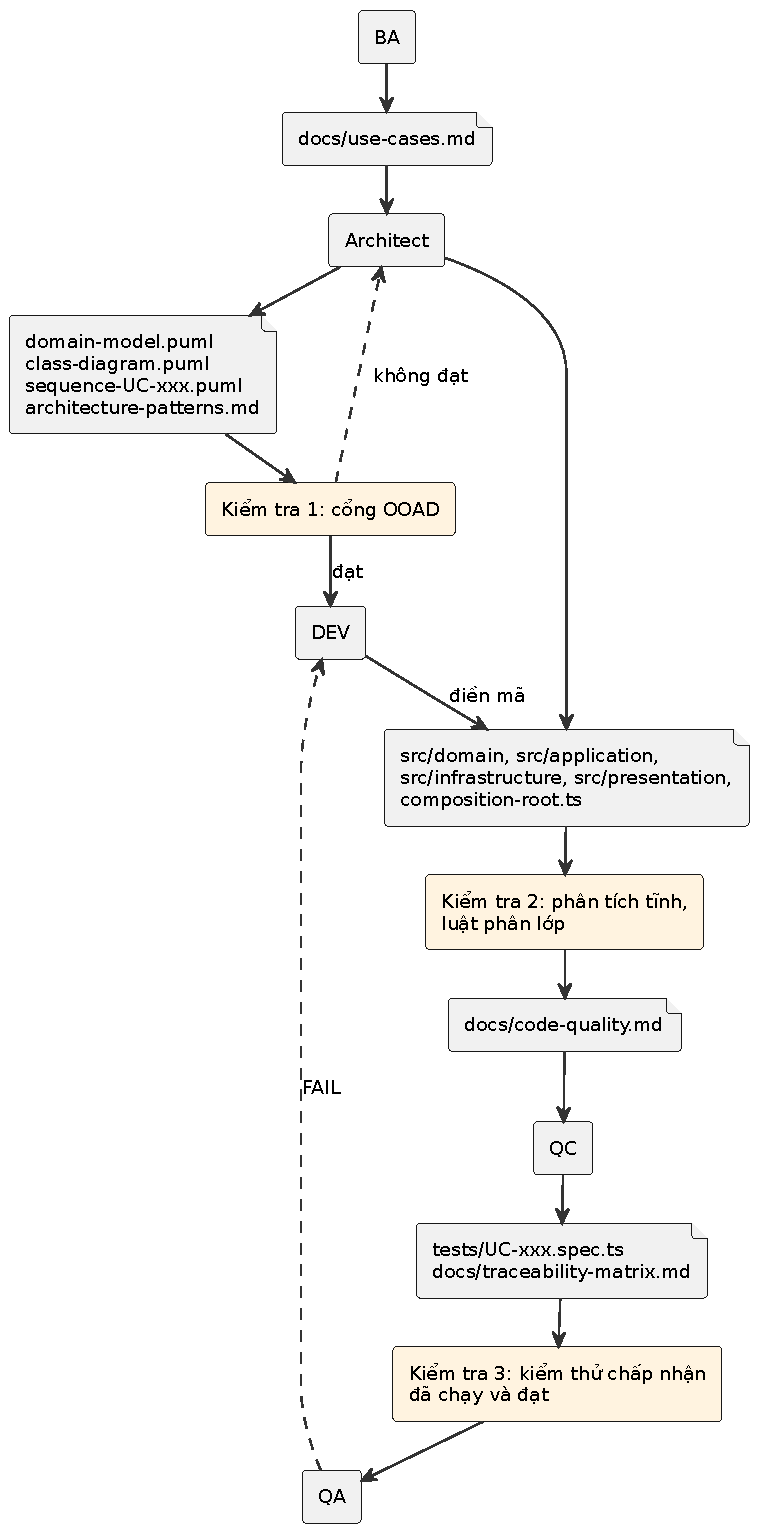
\includegraphics[height=0.6\textheight]{sodo/chuoi-ooad-du-an.pdf}
\end{figure}

\subsection{Ba lớp kiểm tra}

\begin{enumerate}
\item \textbf{Cổng OOAD.} Nút \code{quality_gate} đặt sau bước thiết kế, kiểm tra xem số use case, số thực thể miền, số mẫu thiết kế có đủ ngưỡng không và các tệp bắt buộc đã có chưa. Không đạt thì quy trình quay lại Architect. Mỗi lần đánh giá được ghi vào \code{QualityGateLog} và phát \code{QualityGateEvaluatedEvent}.
\item \textbf{Phân tích tĩnh trước khi QA rà soát} (mục~\ref{subsec:phan-tich-tinh}). Trong đó có luật phân lớp \textit{miền ← ứng dụng ← hạ tầng, trình bày}, theo đó mọi lệnh \code{import} hoặc \code{require()} từ tầng miền sang tầng hạ tầng đều tính là vi phạm.
\item \textbf{Kiểm thử chấp nhận đã chạy.} Độ bao phủ use case chỉ tính những use case có kiểm thử đã chạy và đạt. Use case thiếu kiểm thử hoặc có kiểm thử hỏng được liệt kê đích danh.
\end{enumerate}

Hình~\ref{fig:artifacts} là tab \textit{Artifacts} của một dự án sinh ra. Ở đây người dùng xem được tóm tắt OOAD, kết quả cổng chất lượng, cây tệp, và mở từng sơ đồ đã render. Trong hình đang mở mô hình miền \code{docs/domain-model.puml}.

\begin{figure}{Tab Artifacts của dự án Online Bookstore}
\label{fig:artifacts}
\centering
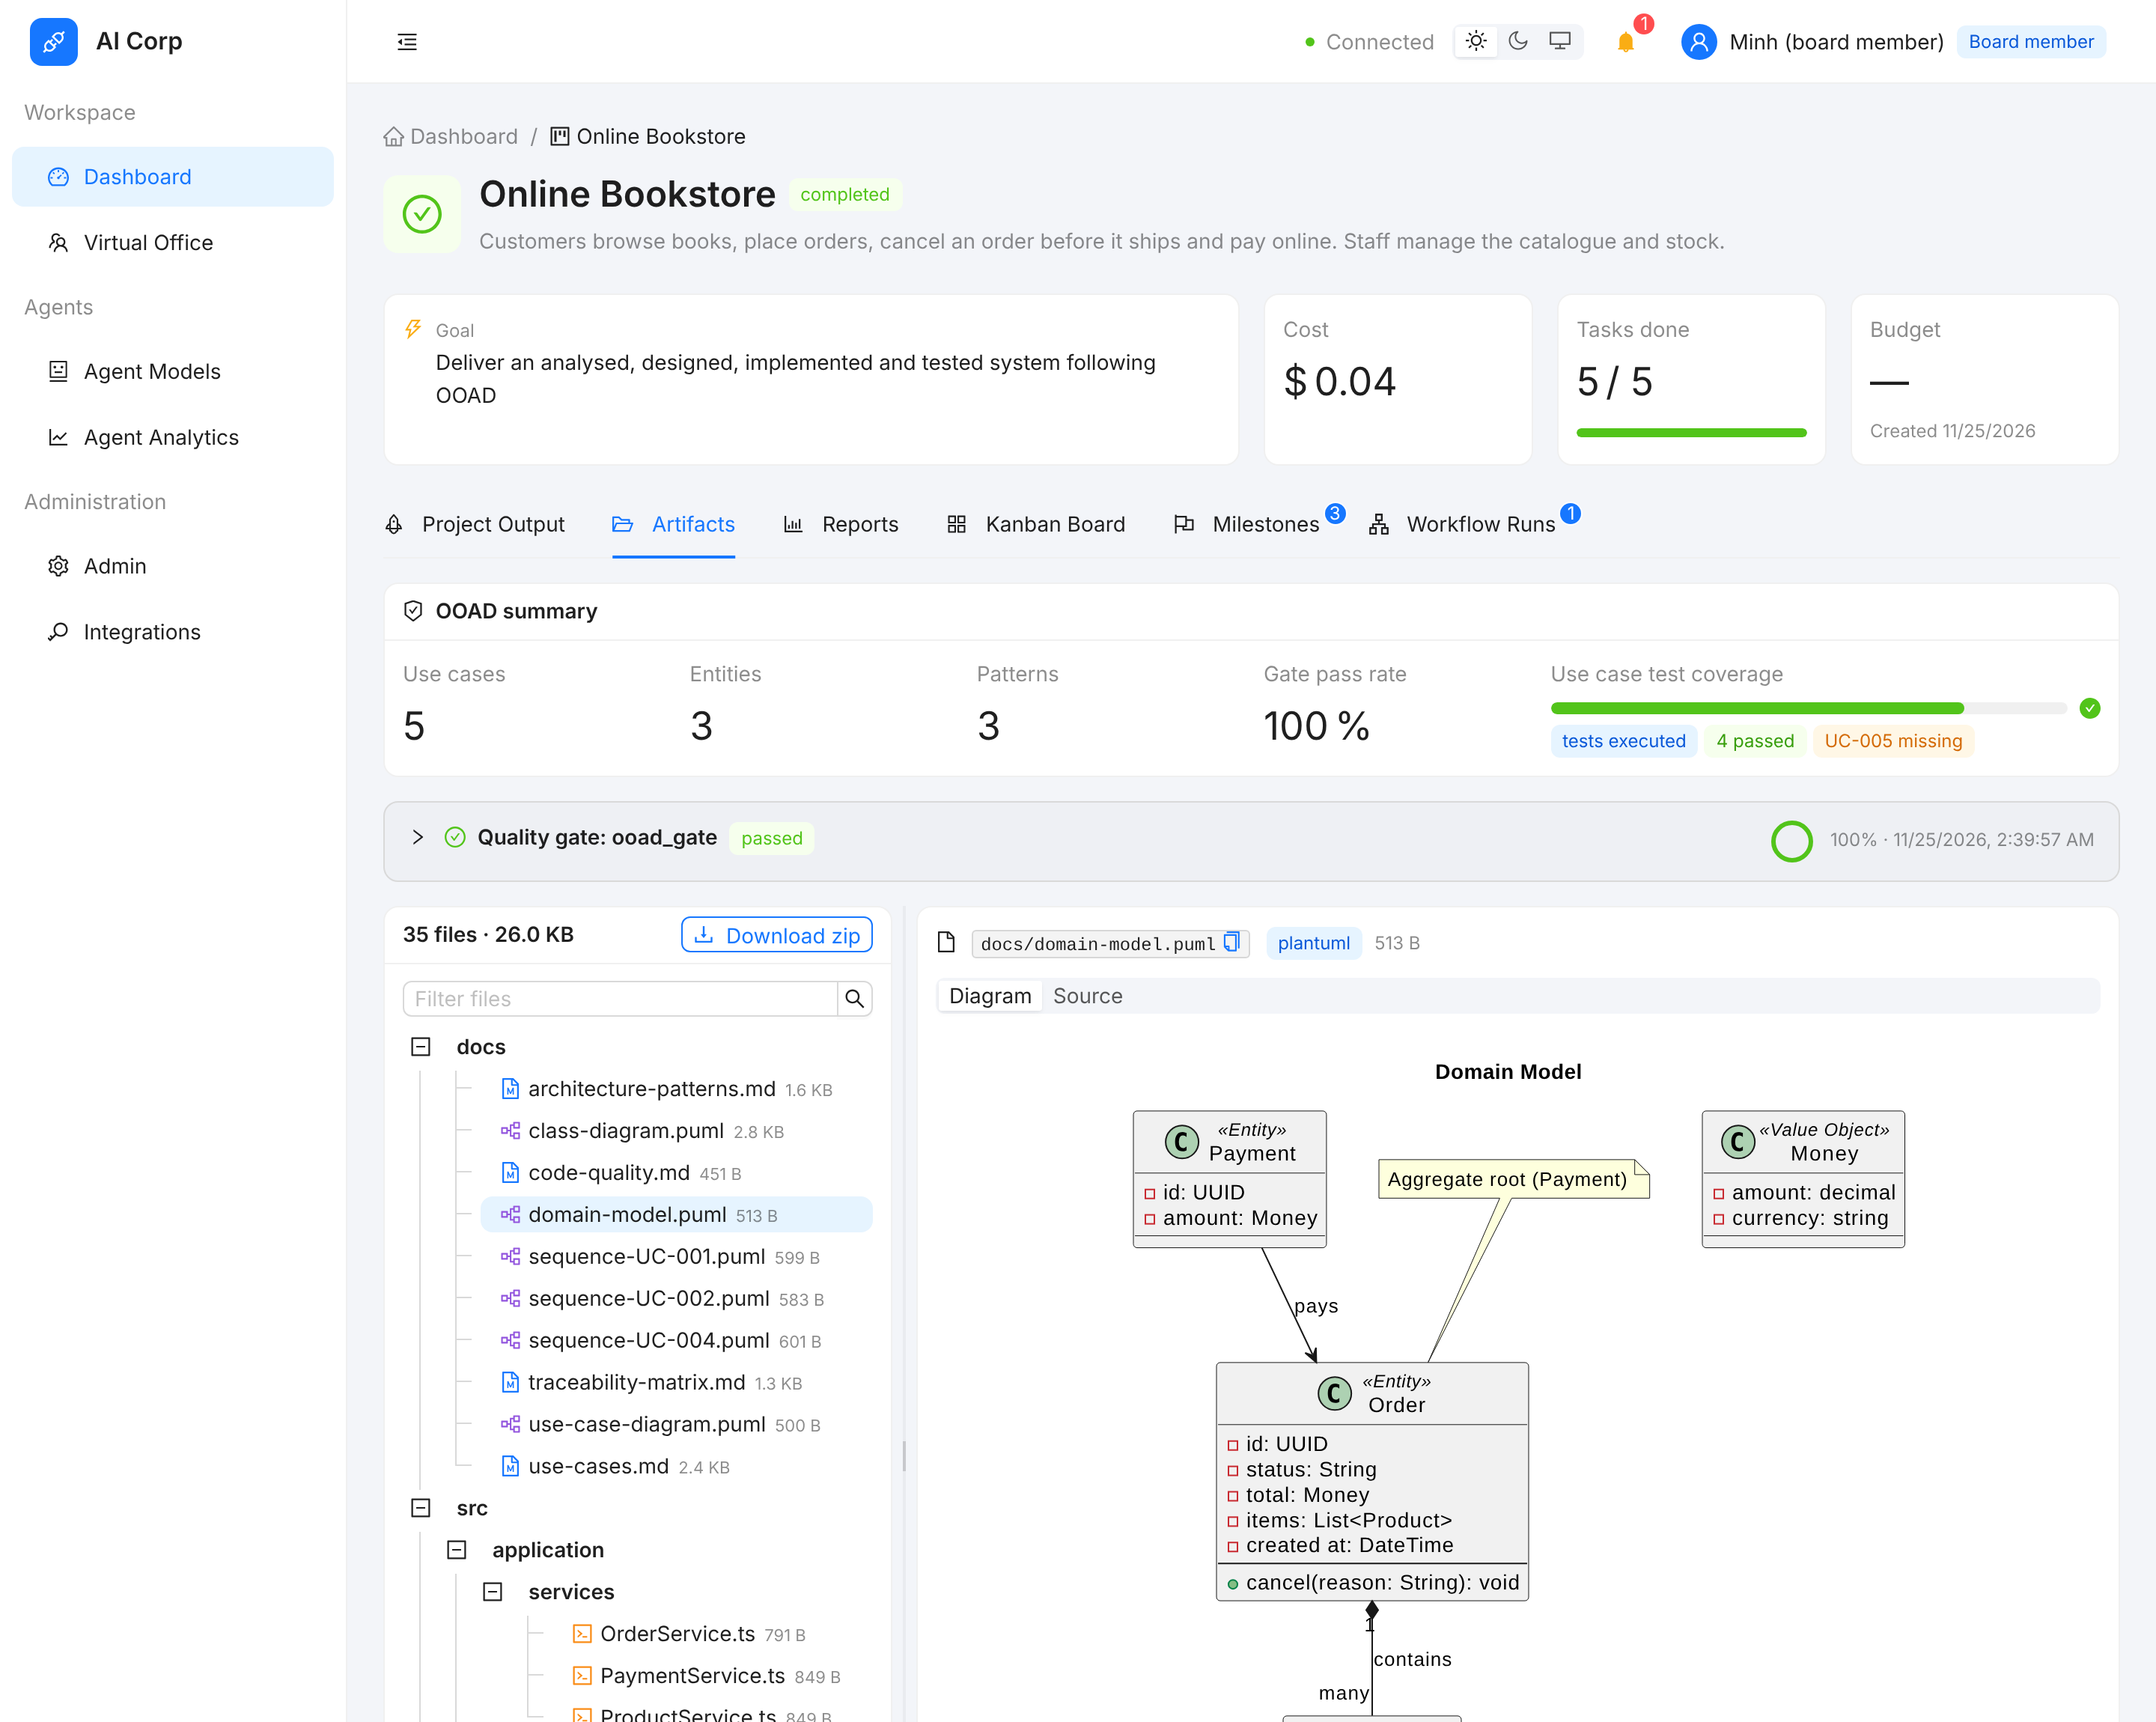
\includegraphics[width=\textwidth]{anh/artifacts.png}
\end{figure}

\section{Bảo mật và tính năng doanh nghiệp}

\begin{itemize}
\item \textbf{Chuỗi guard toàn cục} theo mẫu Chain of Responsibility (Hình~\ref{fig:guard}): \code{AuthenticationGuard} xác thực JWT~\cite{rfc7519} cho người dùng hoặc khoá API cho nhóm \code{/api/v1}, sau đó tới \code{RateLimitGuard}, rồi \code{PermissionGuard}. Mặc định route nào cũng phải đăng nhập, route công khai phải gắn \code{@Public} rõ ràng.
\item \textbf{Quyền của chủ dự án.} \code{AuthorizationService} kiểm tra chủ dự án và người được giao phê duyệt, sai thì trả 403 và ghi \code{access.denied}. Tạo và sửa công việc cũng kiểm tra quyền chủ dự án như khi sửa dự án.
\item \textbf{Đặc quyền tối thiểu khi đăng ký.} Tài khoản tự đăng ký chỉ nhận vai trò người xem (\code{SIGNUP_ROLE}). Quản trị viên nâng quyền ở trang quản lý người dùng và có thể tắt đăng ký (\code{ALLOW_REGISTRATION=false}). Phiên đăng nhập hết hạn sau \code{JWT_EXPIRATION}, mặc định 8 giờ.
\item \textbf{Nhật ký kiểm toán chỉ ghi thêm.} Decorator \code{@Audited} cùng \code{AuditInterceptor} ghi hành động của người dùng, còn \code{AuditLogHandler} ghi hành động của hệ thống và tác tử từ sự kiện miền. Mật khẩu, token, bí mật và khoá được che trước khi ghi.
\item \textbf{API tích hợp.} Khoá API chỉ mang những phạm vi mà vai trò hiện tại của chủ khoá cho phép, tức giao của hai tập phạm vi. Mỗi khoá có giới hạn tần suất riêng. Tài liệu OpenAPI nằm ở \code{/api/docs} và tắt được ở production.
\item \textbf{Webhook.} Payload được ký HMAC-SHA256~\cite{rfc2104} kèm dấu thời gian. URL trỏ vào mạng nội bộ bị từ chối, kể cả khi chỉ lộ ra sau bước phân giải DNS, để chống tấn công SSRF~\cite{owasp2021}. Gửi lại khi lỗi theo thời gian chờ tăng dần.
\item \textbf{Phê duyệt chỉ qua REST.} Quyết định phê duyệt chỉ đi qua \code{POST /api/approvals/:id/approve} hoặc \code{.../reject}, nơi có kiểm tra quyền, kiểm tra người được giao và ghi kiểm toán. Việc trả lời là một cập nhật có điều kiện trên trạng thái \code{pending}, nên hai câu trả lời cùng lúc không thể cùng thành công, và câu thứ hai nhận 409 (Hình~\ref{fig:tuan-tu-phe-duyet}). Quyết định và lý do, bắt buộc khi từ chối, được ghi vào biến của lượt chạy để các tác tử phía sau đọc được.
\item \textbf{Cấu hình production an toàn.} Khi \code{NODE_ENV=production}, API không khởi động nếu thiếu \code{JWT_SECRET} hoặc giá trị này ngắn hơn 32 ký tự, thiếu \code{CORS_ORIGIN}, hay còn giá trị giữ chỗ như \code{CHANGE_ME}. Mọi nơi đọc khoá JWT (REST, guard WebSocket, cổng WebSocket) dùng chung một hàm. Trước đây ba nơi có ba giá trị dự phòng khác nhau, nên khi quên đặt \code{JWT_SECRET}, kết nối thời gian thực luôn bị từ chối.
\end{itemize}

\begin{figure}{Chuỗi guard xử lý một yêu cầu HTTP}
\label{fig:guard}
\centering
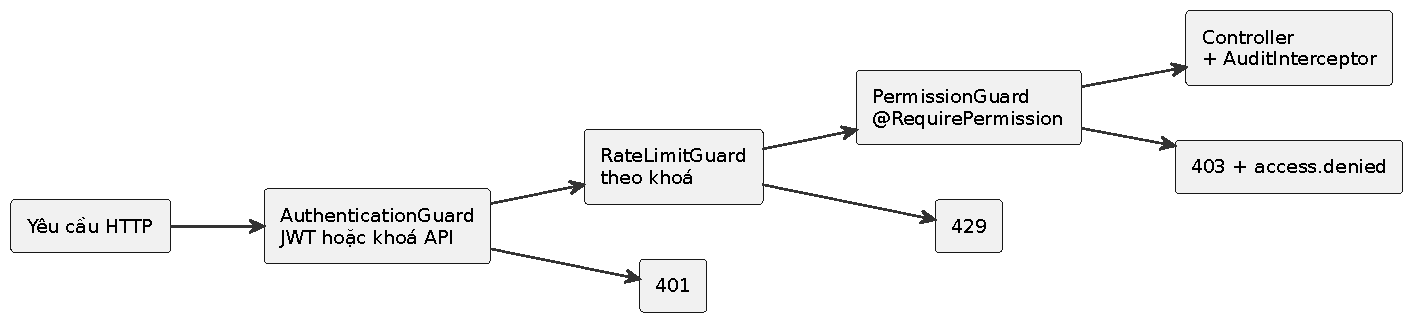
\includegraphics[width=0.9\textwidth]{sodo/chuoi-guard.pdf}
\end{figure}

\begin{figure}{Tuần tự phê duyệt một bước quy trình}
\label{fig:tuan-tu-phe-duyet}
\centering
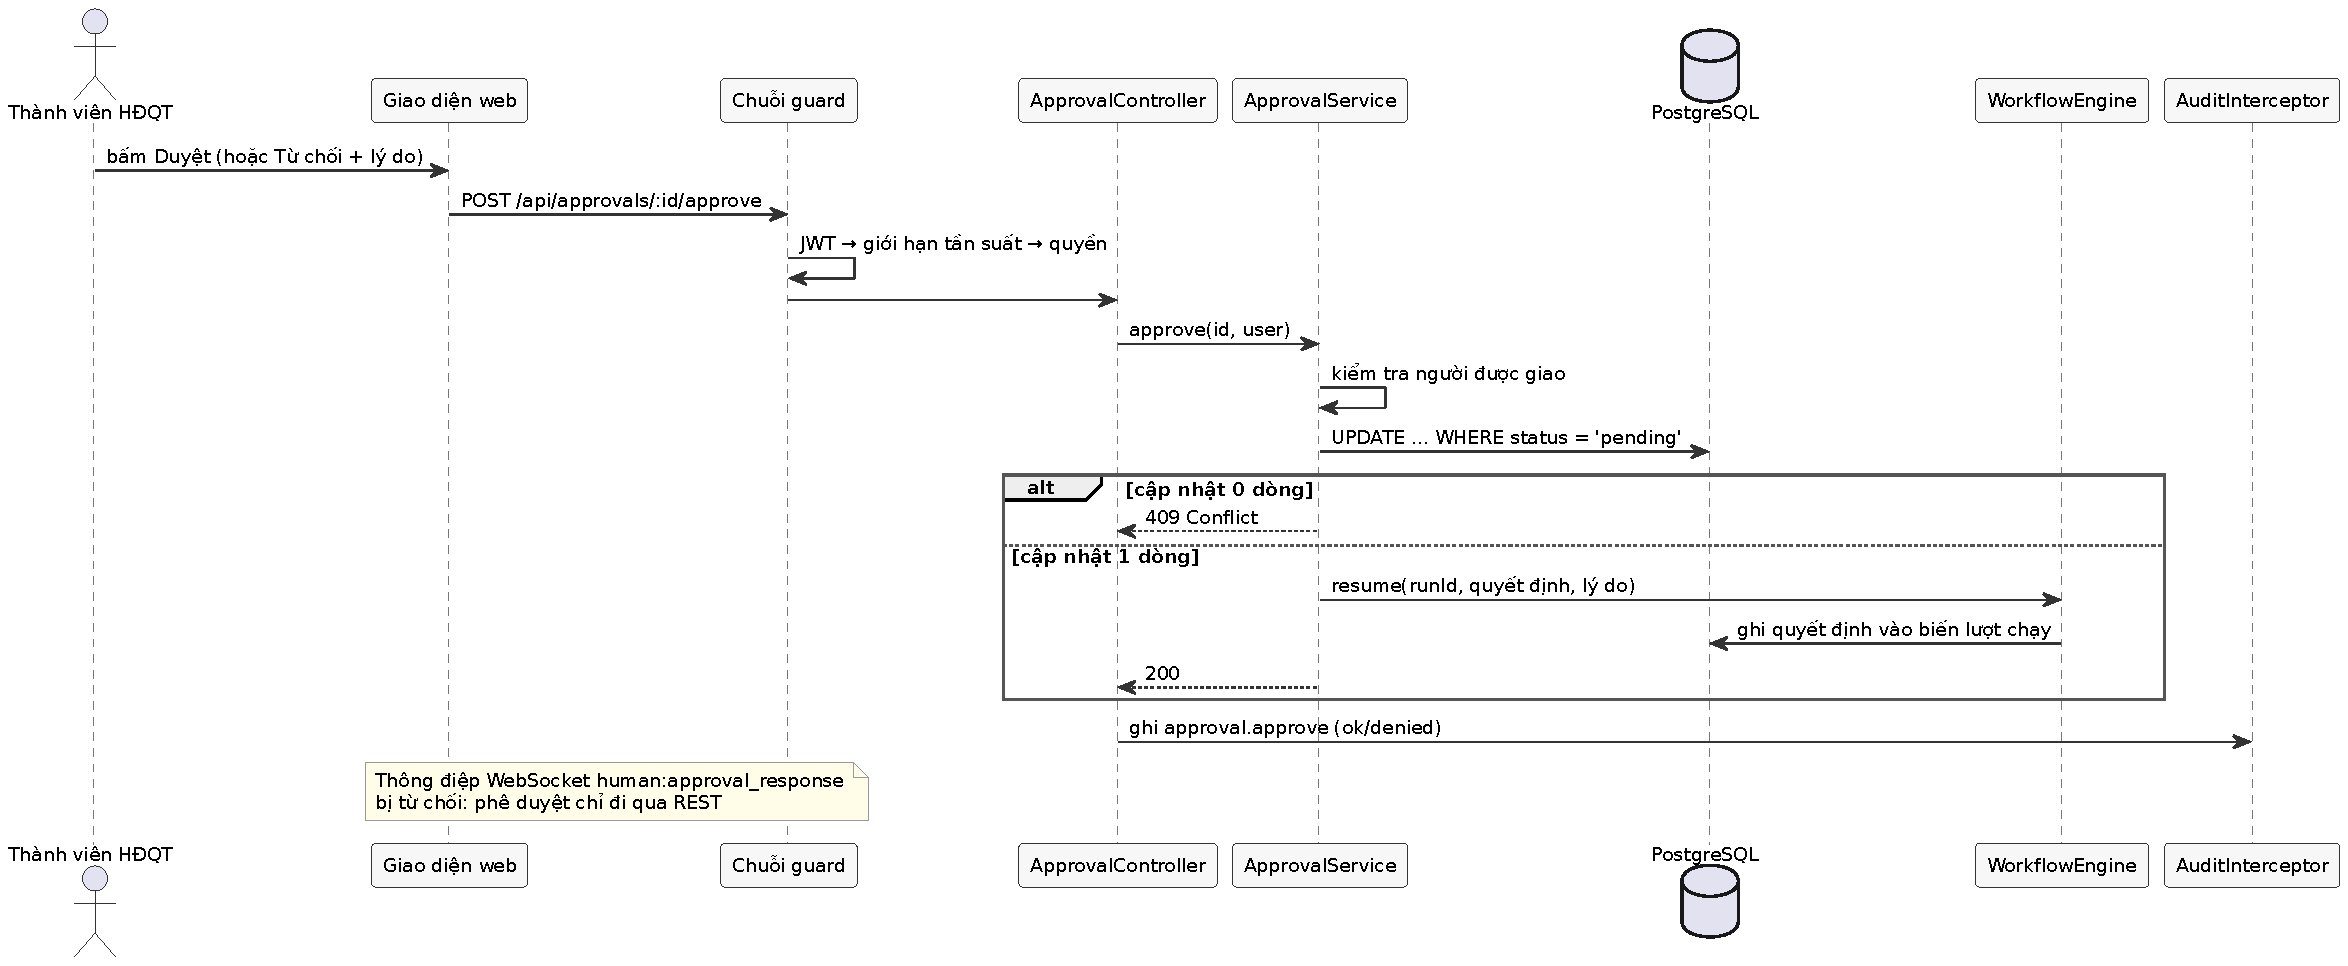
\includegraphics[width=\textwidth]{sodo/tuan-tu-phe-duyet.pdf}
\end{figure}

\section{Phân tích, dự báo và chất lượng mã}

\subsection{Phân tích hiệu năng tác tử}

\code{AgentPerformanceAnalyzer} là một hàm thuần ở tầng miền. Với mỗi vai trò, nó tính số bước, tỉ lệ thành công, thời lượng trung bình và phân vị 95, chi phí cho mỗi lần thành công, điểm chất lượng, xu hướng so với kỳ trước và thứ hạng. Điểm chất lượng không dùng chung một công thức mà đo theo tiêu chí hợp với từng vai trò, qua các \code{IQualitySignal}. DEV tính theo tỉ lệ được QA duyệt, QC theo kết quả kiểm thử, Architect theo kết quả cổng OOAD, các vai trò còn lại theo tỉ lệ đạt ngay lần đầu.

\code{AgentAnomalyDetector} áp năm quy tắc phát hiện bất thường: tỉ lệ thành công giảm 20 điểm phần trăm, ba lần thất bại liên tiếp, chi phí tăng gấp đôi, thời gian chạy tăng gấp đôi và chất lượng dưới 50\%. Mỗi bất thường phát tối đa một lần mỗi ngày qua cùng kênh sự kiện, kiểm toán và webhook.

\subsection{Dự báo thời gian và chi phí}

Nền tảng không chấm giờ công của con người mà ghi thời lượng và chi phí LLM của từng bước tác tử. Do đó mô hình dự báo nhắm vào thời gian của tác tử và chi phí LLM theo từng dự án, từng vai trò, chứ không dự báo giờ công cho từng công việc. Mỗi vai trò có một mô hình hồi quy ridge~\cite{hoerl1970} trên hai đặc trưng là độ dài mô tả dự án và số use case. Vai trò nào có dưới 6 mẫu thì dùng giá trị trung vị. Độ chính xác được báo bằng sai số leave-one-out (MAPE và MAE)~\cite{kohavi1995}, và mỗi dự báo đi kèm một mức tin cậy.

Dự báo được lưu hai lần, một lần khi quy trình bắt đầu và một lần khi PM lập kế hoạch. Xong dự án thì đem so với số liệu thật. Chi phí ước lượng của mỗi công việc PM tạo ra được suy từ dự báo của DEV, QC và QA.

\subsection{Phân tích tĩnh và vòng sửa có giới hạn}
\label{subsec:phan-tich-tinh}

\code{TypeScriptCodeAnalyzer} nằm ở tầng hạ tầng, phía sau cổng \code{ICodeAnalyzer}. Bộ phân tích dùng TypeScript compiler API để tìm lỗi cú pháp. Nó tính độ phức tạp McCabe của từng hàm~\cite{mccabe1976}, thể tích Halstead~\cite{halstead1977} và chỉ số bảo trì đã chuẩn hoá~\cite{oman1992,coleman1994}. Nó cũng tìm lời gọi nguy hiểm như \code{eval} hay \code{Function}, bí mật viết cứng trong mã, vi phạm phân lớp, và gom các chỗ tham chiếu tới use case.

\code{CodeQualityPolicy} ở tầng miền trừ điểm cho từng loại vấn đề, mỗi loại có mức trừ tối đa, rồi lấy trung bình có trọng số theo số dòng. Chính sách dự đoán QA sẽ trả \textit{fail} khi điểm dưới 70, khi có lỗi cú pháp hoặc khi có vi phạm phân lớp. Nếu dự đoán là \textit{fail}, DEV được sửa đúng một vòng, có kèm danh sách vấn đề, và bản sửa chỉ được giữ khi điểm tăng. Khi rà soát, QA dùng báo cáo phân tích làm bằng chứng. Về sau dự đoán này được đem so với phán quyết thật để đo độ chính xác.

\section{Thiết kế triển khai}

Hệ thống được triển khai bằng Docker Compose trên một máy chủ (Hình~\ref{fig:trien-khai}). nginx phục vụ ứng dụng web và làm proxy ngược cho \code{/api}, \code{/socket.io}, \code{/plantuml}. API chạy trên Node~20, khởi động thì chạy migration trước rồi mới nhận yêu cầu. Ngoài ra còn có PostgreSQL kèm pgvector, Redis ở chế độ AOF và một máy chủ PlantUML nội bộ. Kho tệp các dự án là một volume. Chỉ nginx mở cổng ra ngoài. Hồ sơ \code{demo} chạy kèm LLM kịch bản để trình diễn khi không có mạng.

API có hai điểm kiểm tra tình trạng (health check) theo gợi ý của Nygard~\cite{nygard2018}. \code{/api/health/live} cho biết tiến trình còn sống và được Docker dùng làm HEALTHCHECK. \code{/api/health} cho biết hệ thống đã sẵn sàng phục vụ hay chưa. Nó trả 503 khi mất kết nối cơ sở dữ liệu và trả trạng thái \textit{degraded} khi mất Redis hoặc cổng LLM.

\begin{figure}{Sơ đồ triển khai}
\label{fig:trien-khai}
\centering
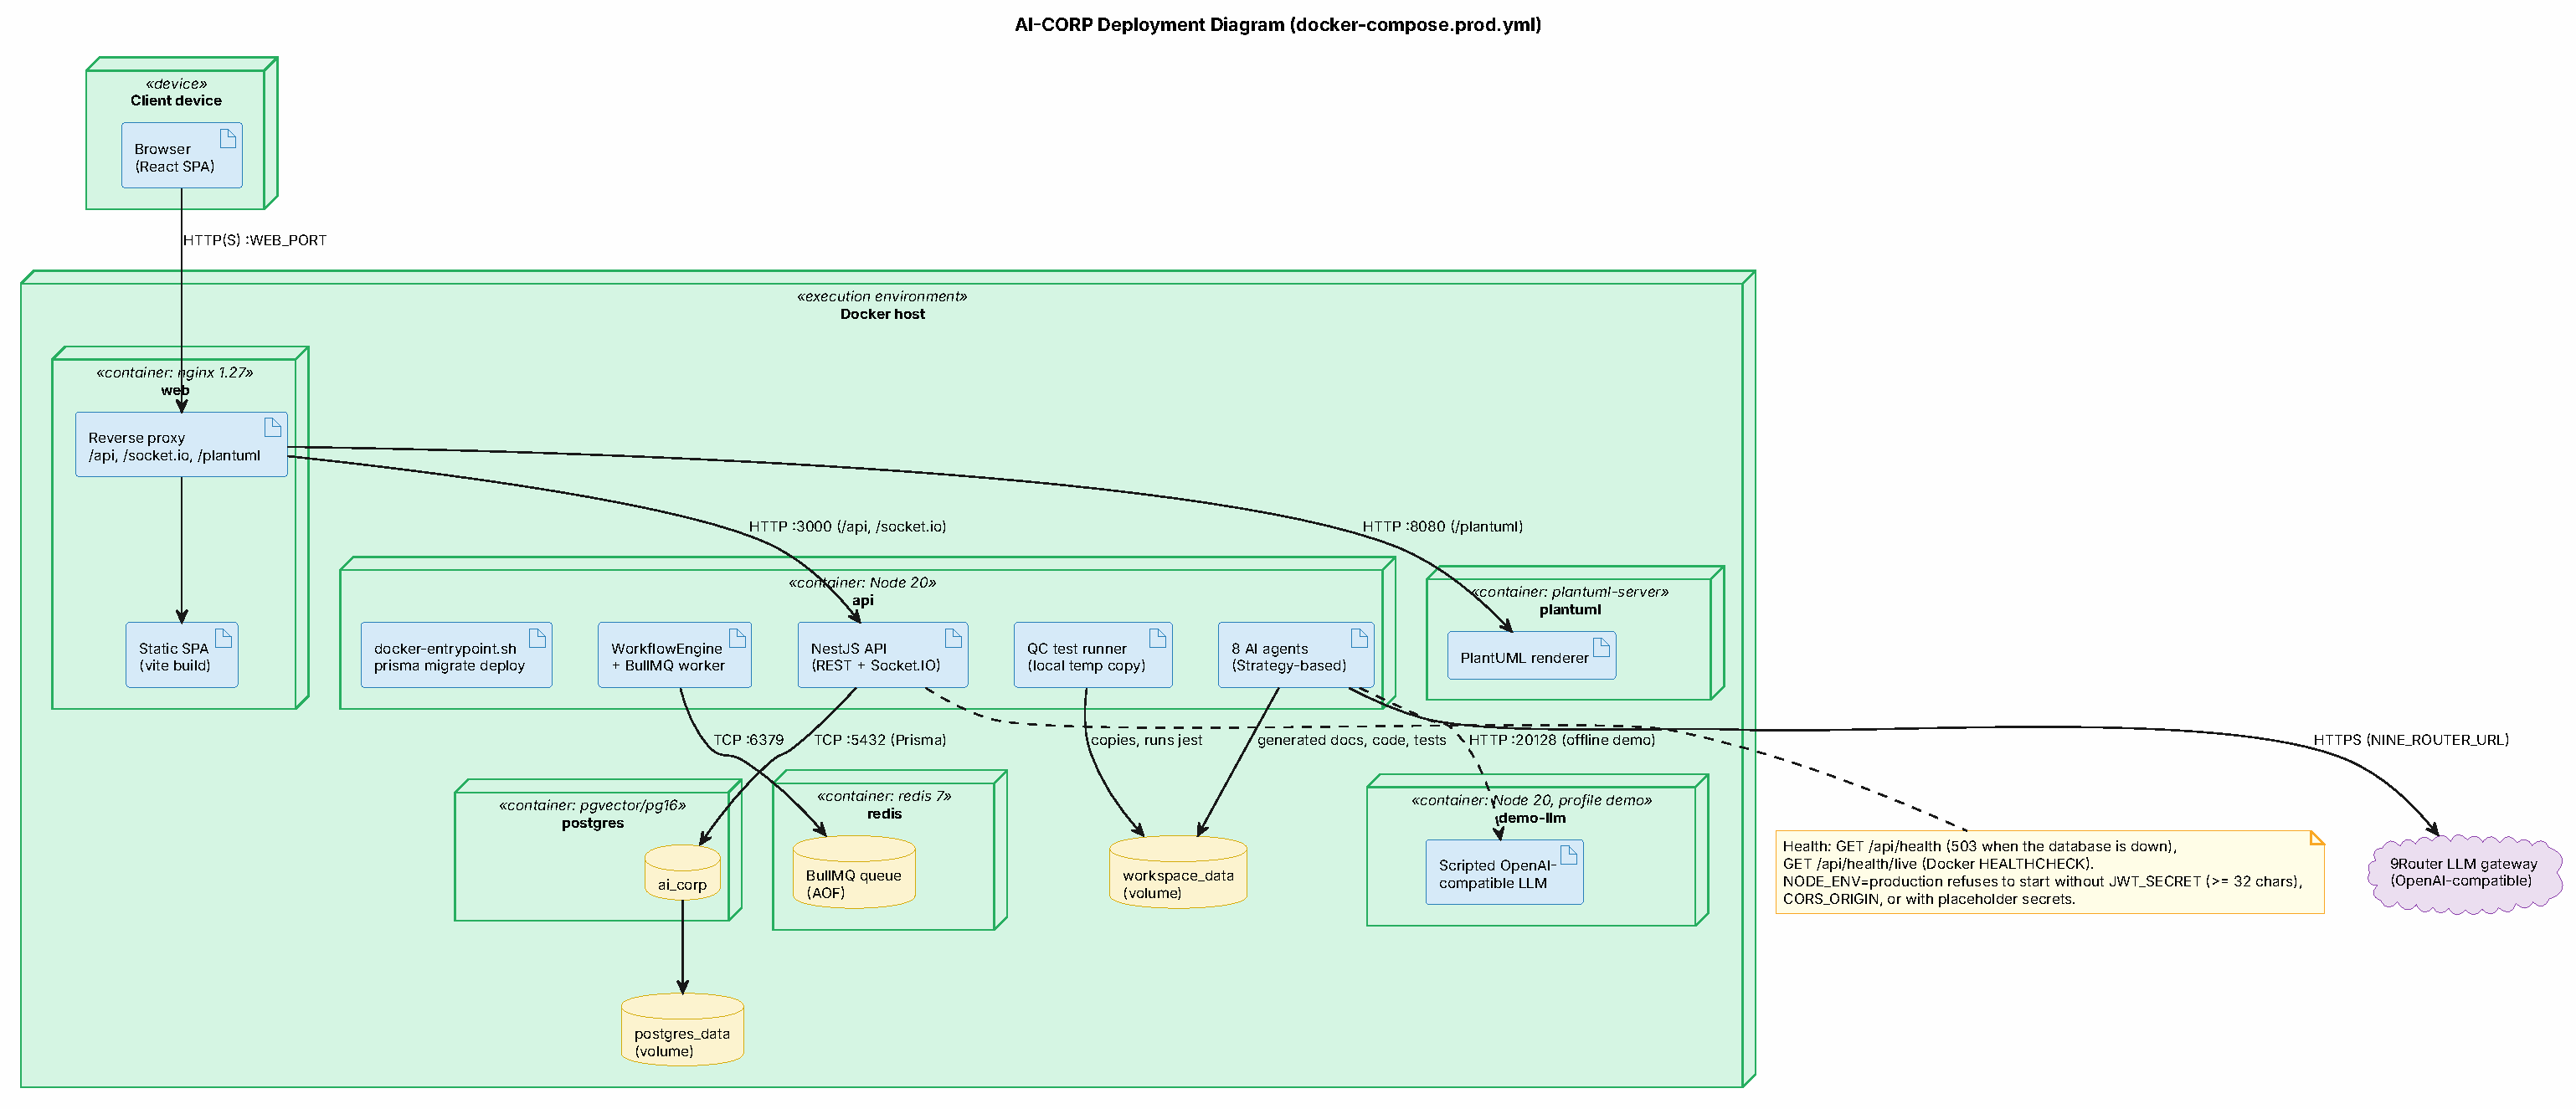
\includegraphics[width=\textwidth]{uml/deployment-diagram.pdf}
\end{figure}
